
\section{Introduction}

In the end of section ~\ref{chp:SOLO_Quite_time}, \citet{Mason-2021-SolOQuietTime} reports the radial gradient of \ac{ACR} oxygen and helium-4 with energy of 4.4 MeV/nuc inside 1 au. The results are based on the measurement in 2020 and the intensities of particle are plotted as a function of three radial gradients. Though the relative larger uncertainty which is due to the limited count number, the results suggest a positive and small oxygen gradient, compared with the observation from Helios and \ac{PSP} \citep{Rankin2021ApJ,Marquardt2018AA}.

As of 2023, \ac{SolO} has finished its fifth orbit and continues its trip in the inner heliosphere and \ac{EPD} provides more measurements for the study of \ac{ACR} radial gradient of \ac{ACR}. 
In this chapter, we will employ the new data from \ac{HET} onboard \ac{SolO} and present the first observation of the \ac{ACR} heliums in the inner heliosphere between 2020 and 2022. Possible interuptions including \acp{SEP}, periodically appeared compression regions and the long term solar modulation are properly considered. Moreover, the helium flux measured by \ac{EPHIN} onboard \ac{SOHO} is utilized to derive the ratio of \ac{SolO} and \ac{SOHO}/\ac{EPHIN} in order to remove the effect of solar modulation. Our preliminary results show that \ac{SolO} and \ac{SOHO}/\ac{EPHIN} are consistent with each other and the radial gradient of helium-4 is closed to the previous results determined by \ac{PSP}, considering the uncertainty.

The details of the data analysis and summary of the results are given below, although some results are still in the preliminary phase. We will continue the data analysis and the final version of the paper is in preparation and to be submited to Astronomy and Astrophysics.


\section{Background}

The \ac{ACR} are the energetic ionized neutrals that widely exist in the heliosphere and dominated the energy of tens of MeV/nuc. The source of \ac{ACR} is believe to be the blunt temination shock located at the boundary of heliosphere.[\citation]. Since the \ac{ACR} was first discovery in 1970, scientists have confirmed the observations of \ac{ACR} helium, oxygen, neon, and also protons in the outer heliosphere. 

The transport of those cosmic ray in the heliosphere is still an unsolved question. When traveling inward, the cosmic rays get modulated by the solar wind and the embedding large scale solar magnetic field. The interactions that affection the propagation of particles in the heliosphere include (a) diffusion caused by the irregular magnetic field, (b) adabitic energy loss and convection due to the expanding solar wind,  (c) gradient and curature drift leaded by the heliospheric magnetic field
Though the cosmic ray transport equation have generally described and modeled those basic processes, the detailed roles of each components in the inner heliosphere and how the new measurement affected by the variable solar magnetic field are still not fully understood. \citep{Rankin2021ApJ}

Particulary the spatial gradient contains the valuable insight of the drift variation of the charged particle through the consecutive solar cycle. As illustrated by \citet{Jokipii1977ApJ, Jokipii1979ApJ, Potgieter2013LRSP}, the drift direction of energetic particle are different during opposite solar polarity, which reverses every $\sim$ 11 years and caused the $\sim$ 22-year cycle. Taking the recent solar minimum (\ac{SC} 24/25, 2020) as an example, the solar magnetic field are in the positive polarity age. The positively charged ions drift inward from the south and north pole region and outward out of the heliosphere along the equatorial plane through the the current sheet. While the situation is reversed in the opposite polarity, the ions drift inward from the equator and leave from the poles. Of course the drift behaviour of electrons are opposite to the ions.

Such a drift effect is reflected in the spatial gradient. The previous observtion by Voyager, Pioneer have found that the latitudinal gradient change sign in two consecutive solar cycles which belong to different polarity.
The comparison between most recent observtion from \ac{PSP} and history observations indicate the different magnetitude of radial gradient between different polarity solar cycle. Despite of this, the precious radial gradient of the current solar cycle especially during the ininial phase of the new solar cycle are not measured and determined.
The radial gradient could be express as \cite{Rankin2021ApJ} :
\begin{equation}
    g_r = \frac{1}{f}\frac{\partial{f}}{\partial{r}} = \frac{\partial{\mathrm{ln} f}}{\partial{r}}
\end{equation}
Where $g_r$ represents the radial gradient component under the assumption that the latitude gradient are neglectable. $f$ is the differential flux and $r$ is the radial distance. The radial gradient could be easily derived by fitting it to a linear equation according to the least minimum square method.


Benefiting from its special orbit with the cloest perihlion at 0.28 au, \ac{SolO} which is launched at the recent solar minimum 24/25 on 2020 provide valuabel insight of the transport effect of the cosmic rays in the inner heliosphere by measuring the radial gradient of those particles.
Below, we present the orbit information of \ac{SolO} from Feb 2020 to May 2023 in Fig.~\ref{fig:SOLO_orbit_info}, which includes the radial distance to the sun, the carrington longtitude and the carrrigton latitude of the \ac{SolO} in the top three panels. As shown in the top panel, the \ac{SolO} has finished five orbits and pass the sixth perihlion moving away from the sun. The closest distance is achived in the fifth cycle on the Sep of 2022. 
The carrington longititude \ac{SolO} indicates the movement of \ac{SolO} related to a fixed longitude line on the sun. Initially the carrington system and its origin point are defined from the Earth's point of view with the mean synodic period of approximately 27.2753 days. While in the \ac{SolO} coordinate becuase the radius of the orbit is not constant, the periods is varying between 26.6 and 35.8 days, slight differing from the period of the Earth.
The latitude is varifing below $\sim$ $\pm$8 degrees.

Besides, we also give the radial distance and the longitudinal seperation between \ac{SolO} and Earth in order to show the relative position of \ac{SolO} to the Earth.

To better visualize and understand the movement of \ac{SolO} in the inner heliosphere and its related position to the sun and the Earth, we draw the orbit track of \ac{SolO} in two different coordinate systems in Fig.~\ref{fig:SOLO_orbit_track}. The left panel show the orbit in helioscentric ecliptic coordinate system, which use the mean equinox as the direction of x axis. \ac{SolO} has an ellipse shape orbit in such a coordinate. On the other hand, in the right panel of Fig.~\ref{fig:SOLO_orbit_track}, the orbit is giving in helioscgraphic coordinate system in which the relative positions of the Sun, the central red point and the Earth, the blue point at 1 au are fixed. The orbits are twisted and changing its shape.

The color bars in both panels indicate the time sequence from Feb 2020 to May 2023. Moreover, the carrington rotation numbers are marked at the start of the each carrington cycle and labeled next to the orbit track. The moving direction of spacecraft can been read from change the number and colors.
%Obviously, when the spacecraft is located away the sun, the \ac{SolO} is moving in a limited region, with hardly changed longtitude in one carrington rotation. Conversely, the longitudinal changes are large when \ac{SolO} rapidly pass by the sun. Between them the radial distance change quickly. 


%In this report, we organized the content as following: We first introduce the data and instrument we used in this work, which including the SOLO/HET, SOHO/EPHIN, STEREO/LET and possiblely LND. In chapter 3 we give the overview of the observation of the helium-4 between 2020 and 2022 when in the second half, SEPs frequently happens and the overall cross-calibration between different instrument

%In section4, we explain the several kind of effect that could disturbe the constanct background and show how the result are affected by different method.  In the end, we conclude.



\begin{figure}
    \centering
    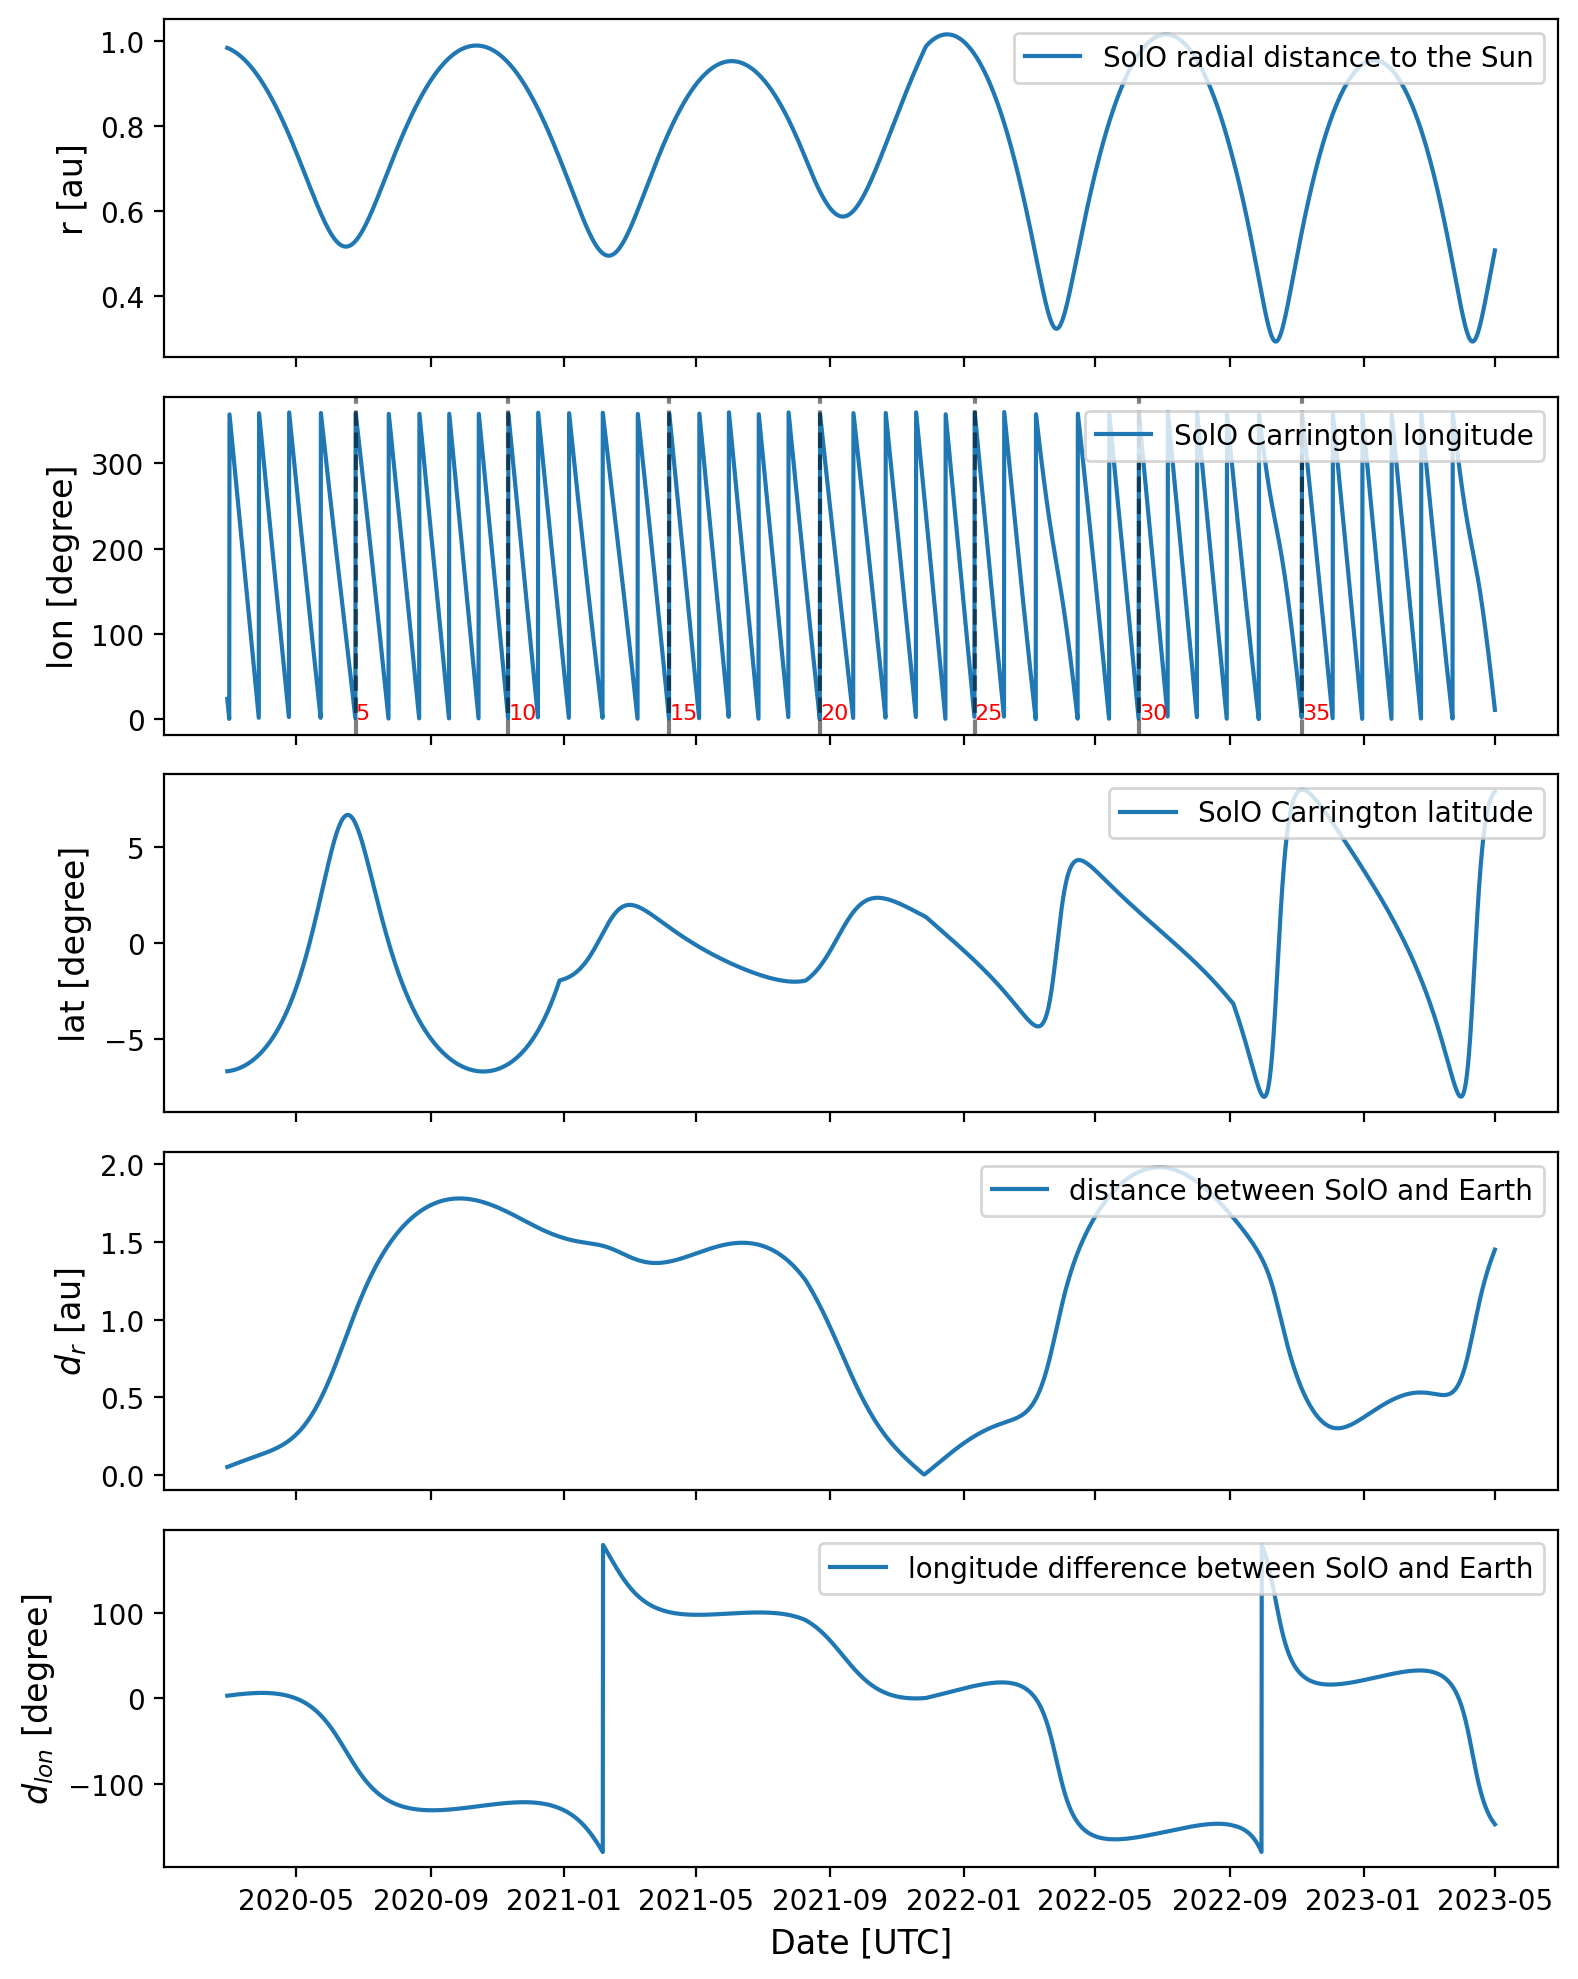
\includegraphics[width = 0.7\textwidth]{images/ACR/SOLO_orbit_helioscentric_3.png}
    \caption[The orbit variation of \ac{SolO} in carrington coordinate system]{(From top to the bottom) The variation of \ac{SolO} radial distance, carrignton longitude, carrington latitude in the carrington coordinate system as well as distance and longitude seperation between \ac{SolO} and \ac{SOHO}. Date is from Feb 2020 to May 2023. }
    \label{fig:SOLO_orbit_info}
\end{figure}
\begin{figure}
    \centering
    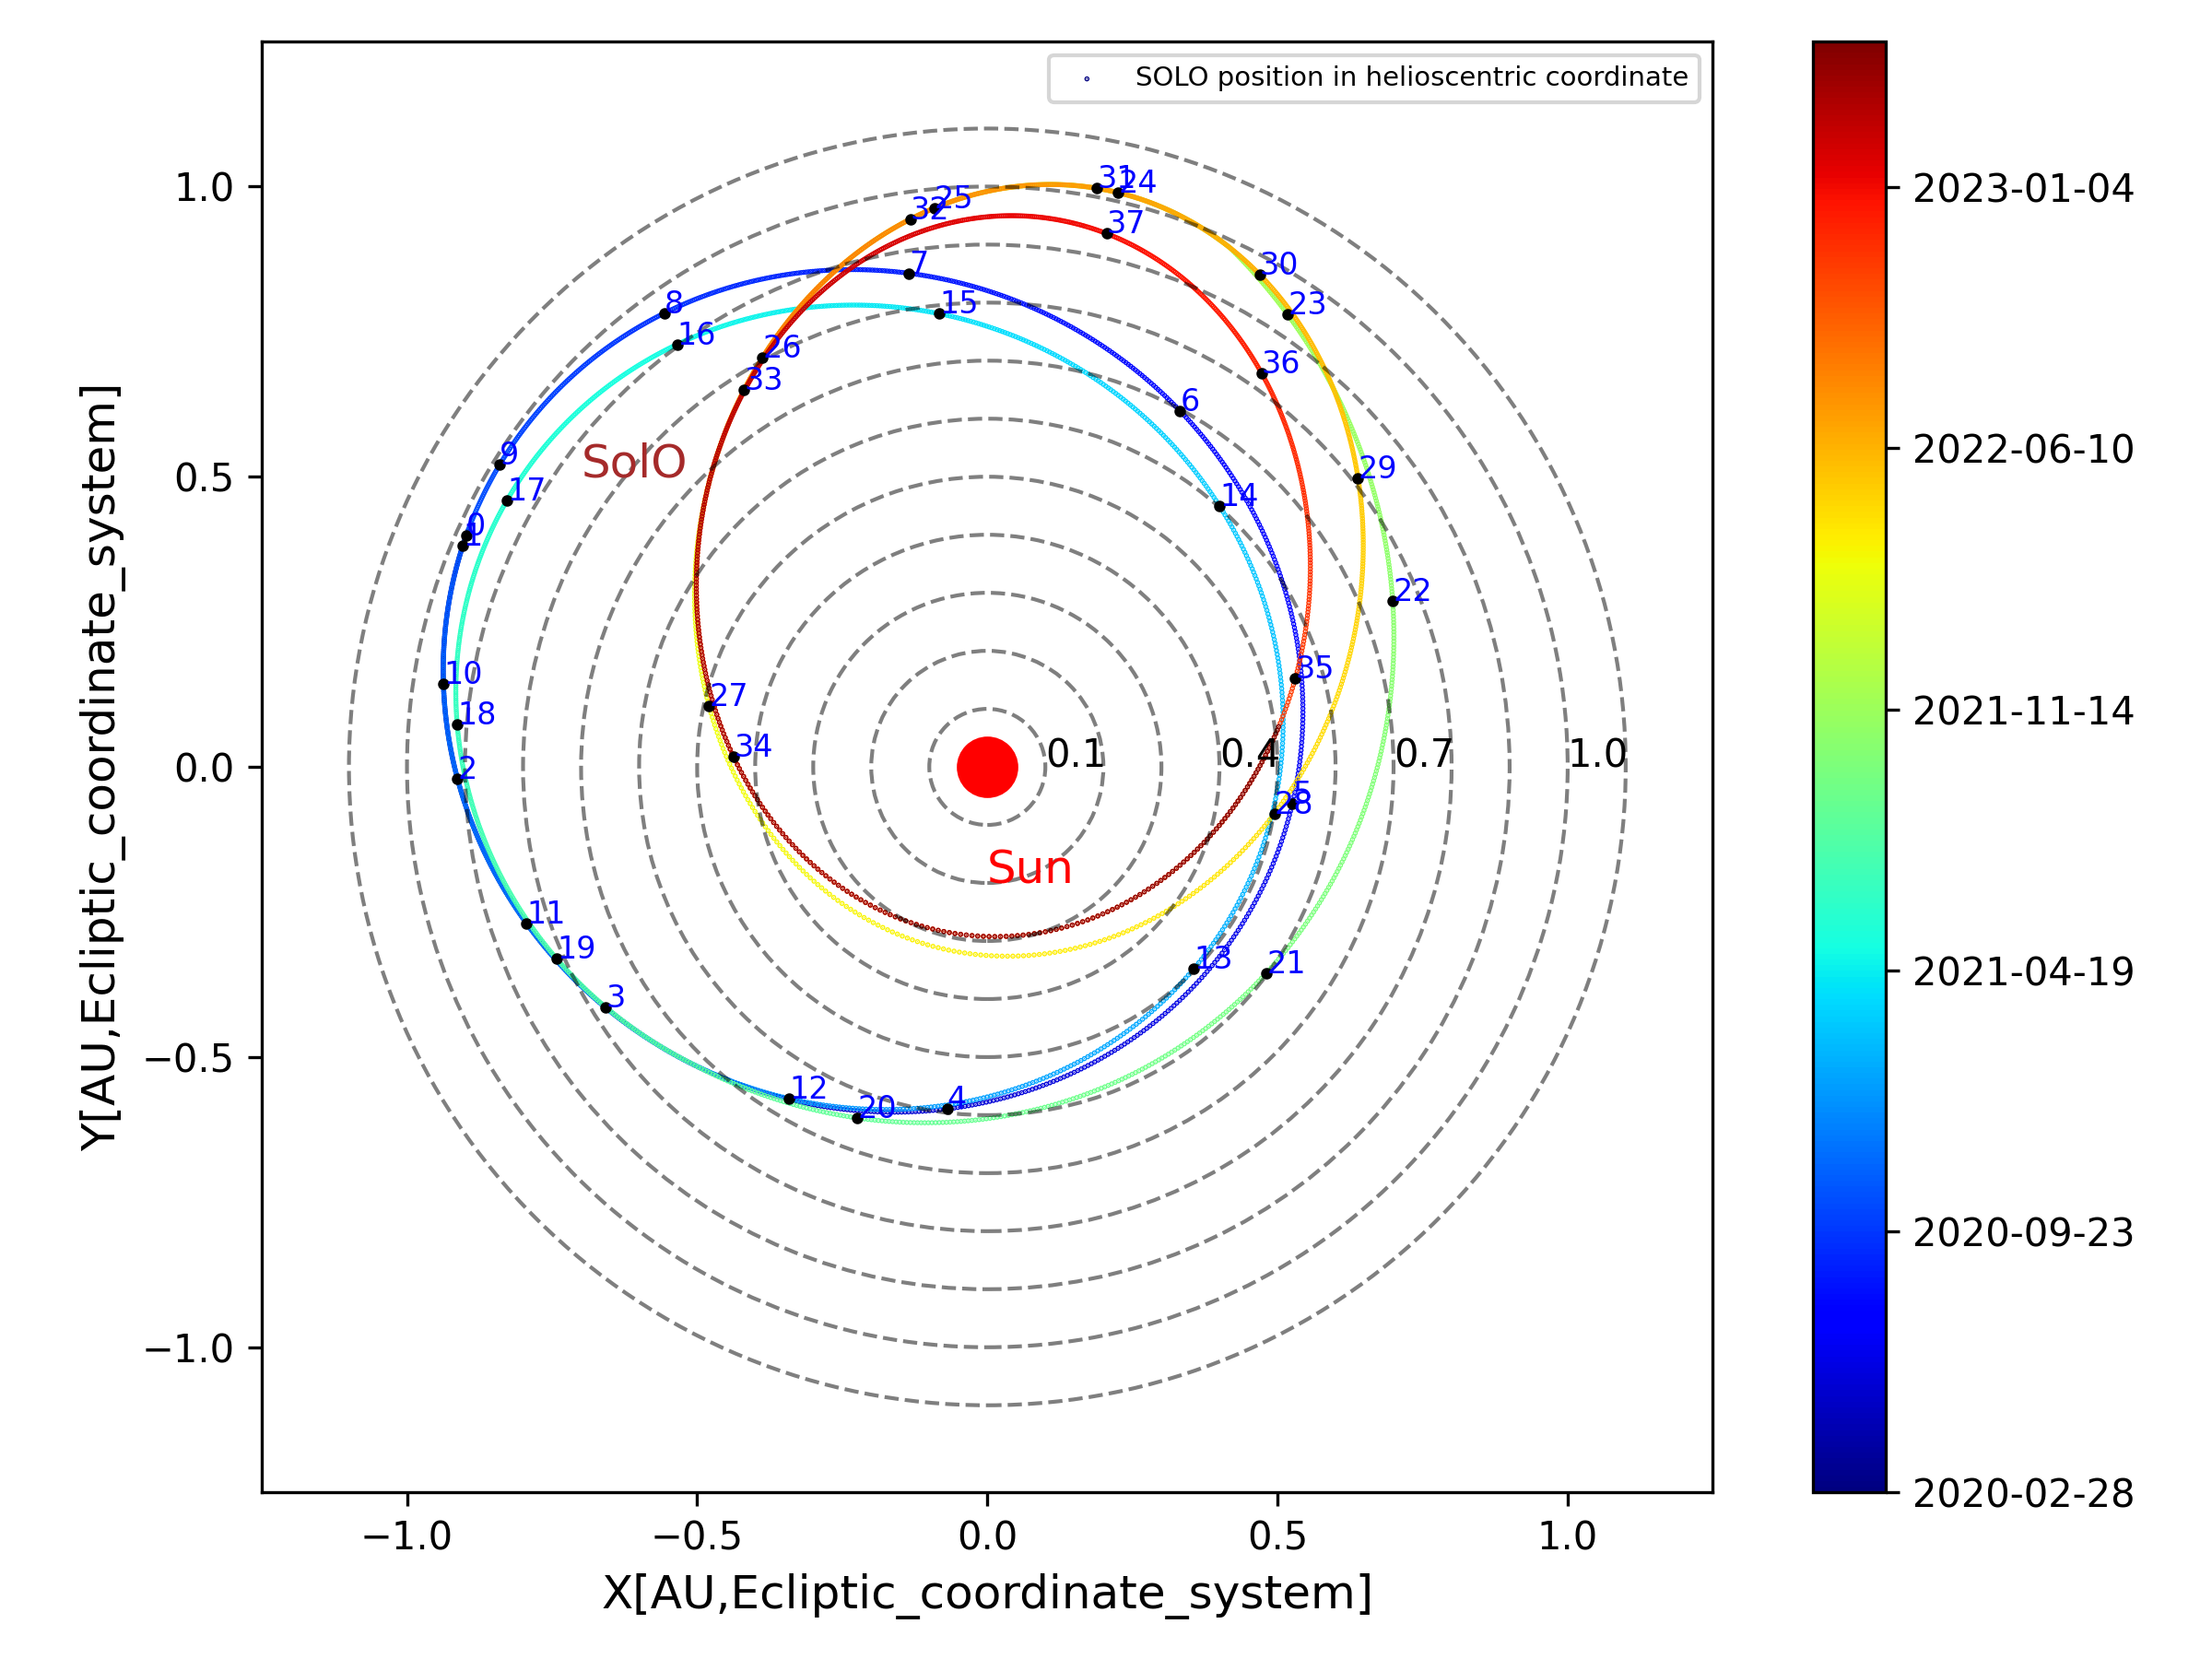
\includegraphics[width=0.45\textwidth]{images/ACR/SOLO_orbit_track_helioscentric_3.png}
    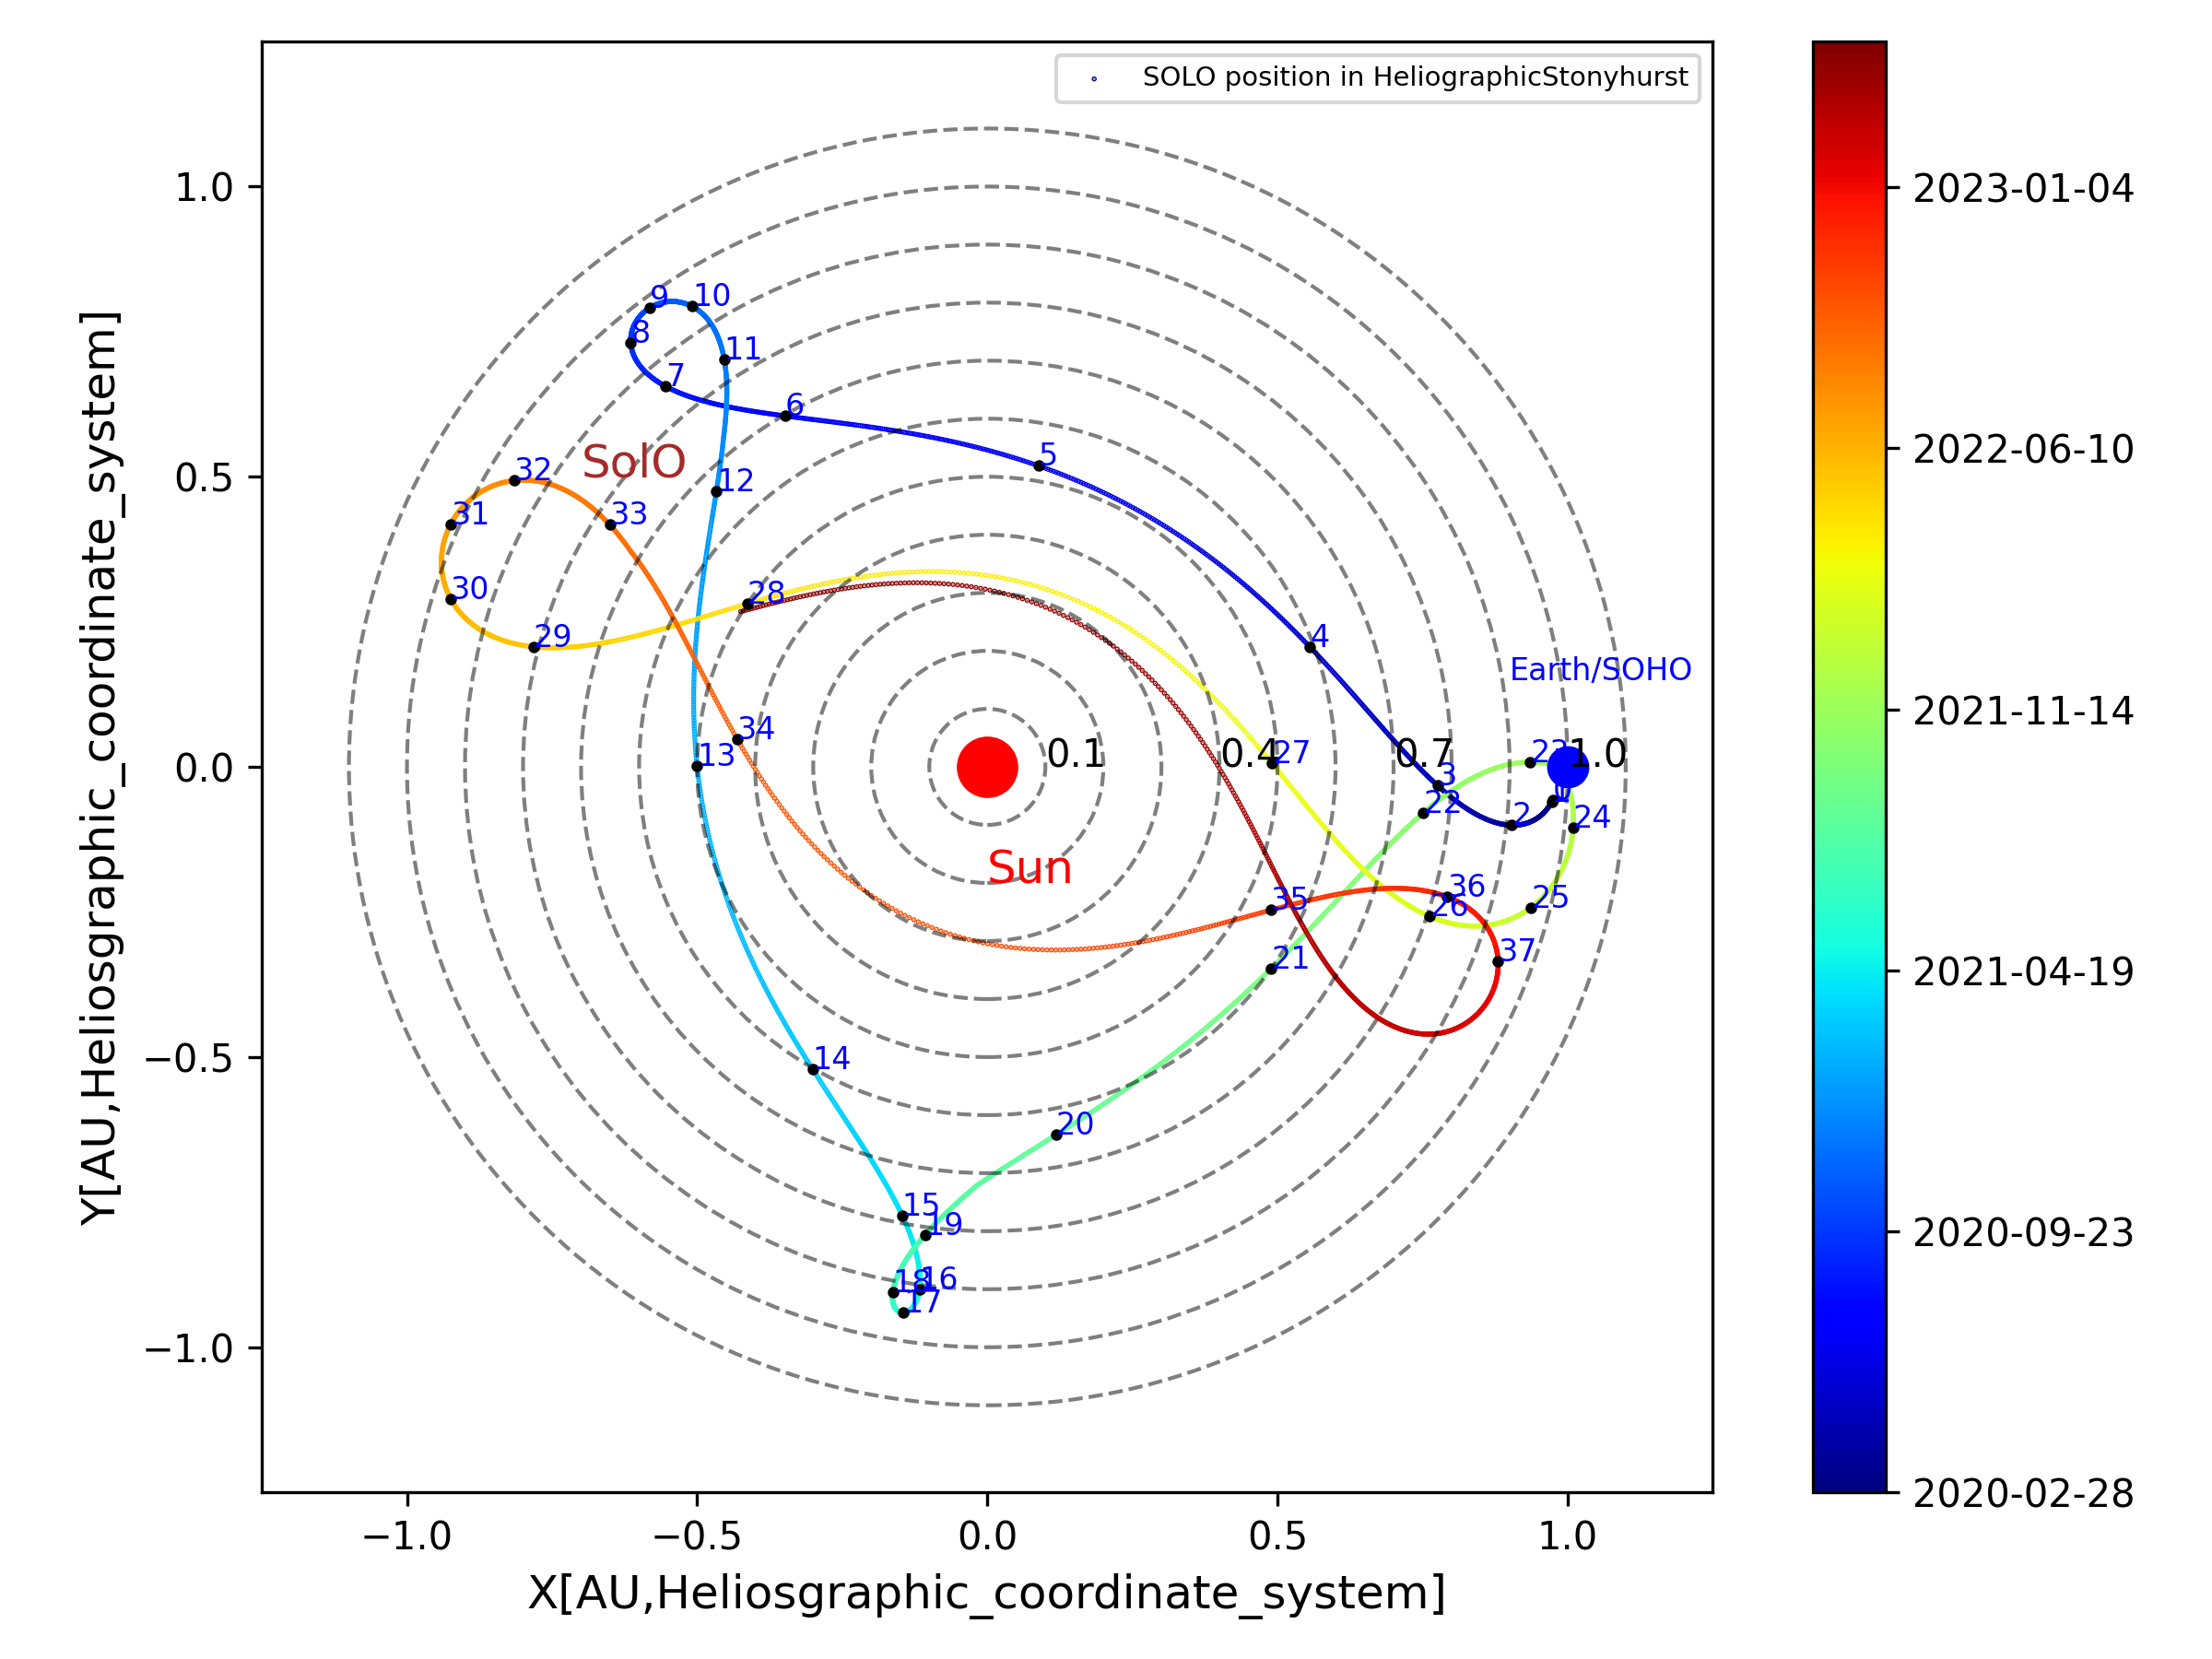
\includegraphics[width = 0.45\textwidth]{images/ACR/SOLO_orbit_stonyhurst_3.png}
    \caption[Orbit track of \ac{Solo}]{Left: The orbit track of \ac{SolO} in the helioscentric mean ecliptic coordinate system where the origin is the center of the sun, and x axis points in the direction of the mean equinox and xy-plane is the ecliptic plane. Right: The orbit track of \ac{SolO} in the stonyhurst coordinate system. The location of Earth at 1 au is marked as the blue solid circle. The numbers next to the track are the carrington rotation periods.
    Date is from Feb 2020 to May 2023.}
    \label{fig:SOLO_orbit_track}
\end{figure}




\section{Instrument}


The particle data reported in this study are mainly from the \acl{HET} onboard \ac{SolO} which measures ions in the energy range from tens of MeV/nuc to hundred MeV/nuc. Particularly, we focus on the heliums of \ac{ACR} energy from 10 MeV/nuc to 50 MeV/nuc. The detials of \ac{HET} can be found in the previous section and \citet{RodriguezPacheco-2019-EPD}.
Similar with \ac{SIS} observation by \citet{Mason-2021-SolOQuietTime}, the analysis of \ac{HET} measured helium is also contrained by their counting statistic due to the limited \ac{HET} geometry factor. In order to increase the count number and reduce the uncertainty, two measures are taken. First, we combined the data from four different directions. \ac{HET} is charaterized with its four apartures pointing to sun, antisun, south and north. By assuming the \acp{ACR} are isotropically distributed, summations of those data could effectively reduce the uncertainty to half. Furthermore, we extend the fine energy bins of \ac{HET} nominal data product and reconstruct the energy channel of particle stopping in C to the following energy range, 10 - 20 MeV/nuc, 20 - 30 Mev/nuc, 30 - 40 Mev/nuc, 40 - 50 Mev/nuc. The exact values of the left and right boundary of bins are determined by the values of nominal data products.

In addition to the nominal data products which are designed to provide precious intensity measurement with high energy resolution, we utilize one type of housekeeping data named any(a1, b1) to determine the \ac{SEP} period using the background and 3-sigma method. Here \textit{a1} and \textit{b1} represent the front two sensor head of \ac{HET} in sun direction. This level-2 trigger counts all  particles with energy above the threshold of detector A or detector B, which is set to 50 keV in the nominal mode \citep{Elftmann-2020-PhD}. This trigger can detect both energetic electron, protons and heavy ions without any elements resolution, making it an ideal indicator of the solar activity and \ac{SEP} with imporved counting statistics. Then we could determine a list of \ac{SEP} by applying the 3-sigma method.

Apart from the measurement from \ac{SolO}, we also utilized the observations from \ac{SOHO}/\ac{EPHIN}, \ac{ACESIS} and \ac{CRIS} onboard \ac{ACE} and \ac{LND} as a comparsion and reference line, in particular when encountering long term variations of the cosmic rays.

\section{Observation and data analysis}

\subsection{Overview observation between 2020 and 2022 and the cross calibration between four instruments}

\subsubsection{Spectra comparison between \ac{HET} and other instruments}

Before we start deriving the radial gradient, we first have a quick overlook of the observation of heavier ions, including helium, carbon, nitrogen and oxygen from \ac{HET}, as Fig.~\ref{fig:overview} shown. After removed the possible \ac{SEP} contaminations, the averaged spectra between 2020 and 2022 are displayed. The \ac{SEP} list are determined below and the completed list of periods that we remove are also given.

We first go through all the data point in this figure.
The \ac{HET} measurements are marked as diamonds of different colors with red for helium-4, blue for oxygen, orange for carbon and green for nitrogen.
All the helium nominal scientific data products from \ac{HET} are presented which include particle stopping in detector B ($<$ 10 Mev/nuc), in detector C (10 - 100 MeV/nuc) and penetrating particles ($>$ 100 MeV/nuc), despite that the penetrating helium will not be used in the later analysis of \ac{ACR} gradient.
The penetrating helium composes of two populations depending on their primary energy, that are the just penetrating helium marked as empty red diamonds and the full penetrating particle with energy above 200 MeV/nuc. 

It is worth noting the potential issue of these penetrating data products. The intensity measured by two channels around 100 MeV/nuc are higher than the nearby channels and current we have no idea of the reason, probably due to the dead layer or because that the channels have not been properly calibrated.
Besides, the geometry factors of fully penetrating particles channels, i.e. the last three channels, are divided by a factor of two, to account for those \acp{GCR} equally incident from opposite directions. The current version of geometry factors are obtained based on the 2$\pi$ simulation by assuming the \ac{SEP} are highly anisotropic and arrive the detector from only one direction. 

The \ac{ACE} measurements are plotted as circles including filled circles representing \ac{ACESIS} and empty one for \ac{CRIS}. Unfortunately, \ac{ACESIS} only measured helium with energy below 15 MeV/nuc.
The helium data from \ac{SOHO}/\ac{EPHIN} are shown as the purple squares and the \ac{LND} measured helium-4 are shown as the brown triangles. Their measurement cover the \ac{ACR} energy range between 10 - 50 MeV/nuc.

The cross-comparison of the averaged spectra of all particle species in Fig.~\ref{fig:overview} reveals a general agreement between different instruments despite their distinct positions. This agreement indicates the reliable measurement of the \ac{SolO} and also \ac{LND}, which we for the first time report the helium-4 spectrum. Futhermore, the flat helium spectra between 10 MeV - 50 MeV/nuc and the higher intensity of oxygen and nitrogen at 10 MeV/nuc clearly demonstrate the presence of the \ac{ACR} components in the inner heliosphere. 
Later in Fig.~\ref{fig:helium_spec_1au}, we specifically focus on the helium-4 spectra based on the measurement when \ac{SolO} was positioned between 0.95 and 1 au. The time periods we selected in the last two years are given in Tabel \ref{tab:1AU_period}, which consist of the start time, end time and the distance from \ac{SolO} to the Earth.
Similarly, the \ac{EPHIN} and \ac{HET} helium of energy above 10 MeV/nuc show  the consistency in averaged spectrum. However, the discrepancy appear on the energy channel below 10 Mev where the intensity of \ac{ACESIS} is about 2 time higher than \ac{EPHIN}. Besides, the \ac{LND} spectrum appears generally higher than the other measurements and it also has larger error bars. This due to the limited operation time on the lunar surface (see section \ref{sec:change_4_LND}). As a result, we utilize the \ac{EPHIN} and \ac{HET} helium measurement within the energy of 10 to 50 MeV/nuc in the susequent analysis.



\begin{figure}
    \centering
    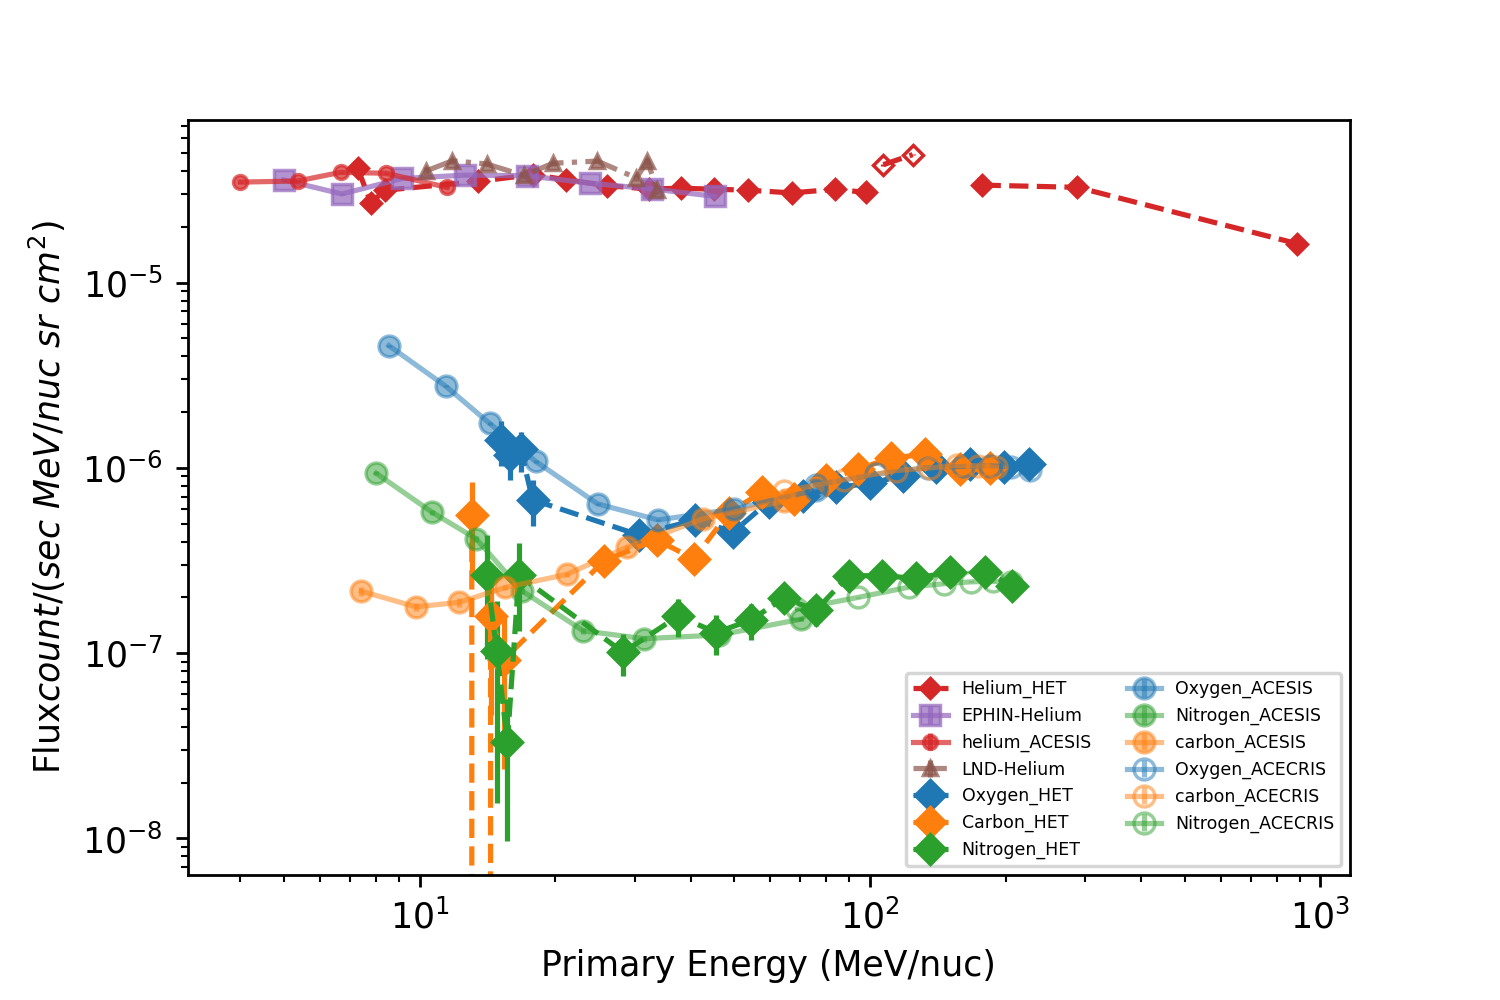
\includegraphics[width = 0.8\textwidth]{images/ACR/ACE_SIS_CRIS_SOLO_all_3.png}
    \caption[The quite time spactra of helium, carbon, nitrogen and oxygen between 2020 and 2022]{The helium-4 (red, brown, purple), carbon (orange), nitrogen (green) and oxygen (blue) spectrum averaged between 2020 and 2022. The \ac{SEP} events are removed. The data used in this figure consist of observation from \ac{SolO}/\ac{HET}, \ac{SOHO}/\ac{EPHIN}, \ac{ACE} and \ac{LND}}
    \label{fig:overview}
\end{figure}
\begin{figure}
    \centering
    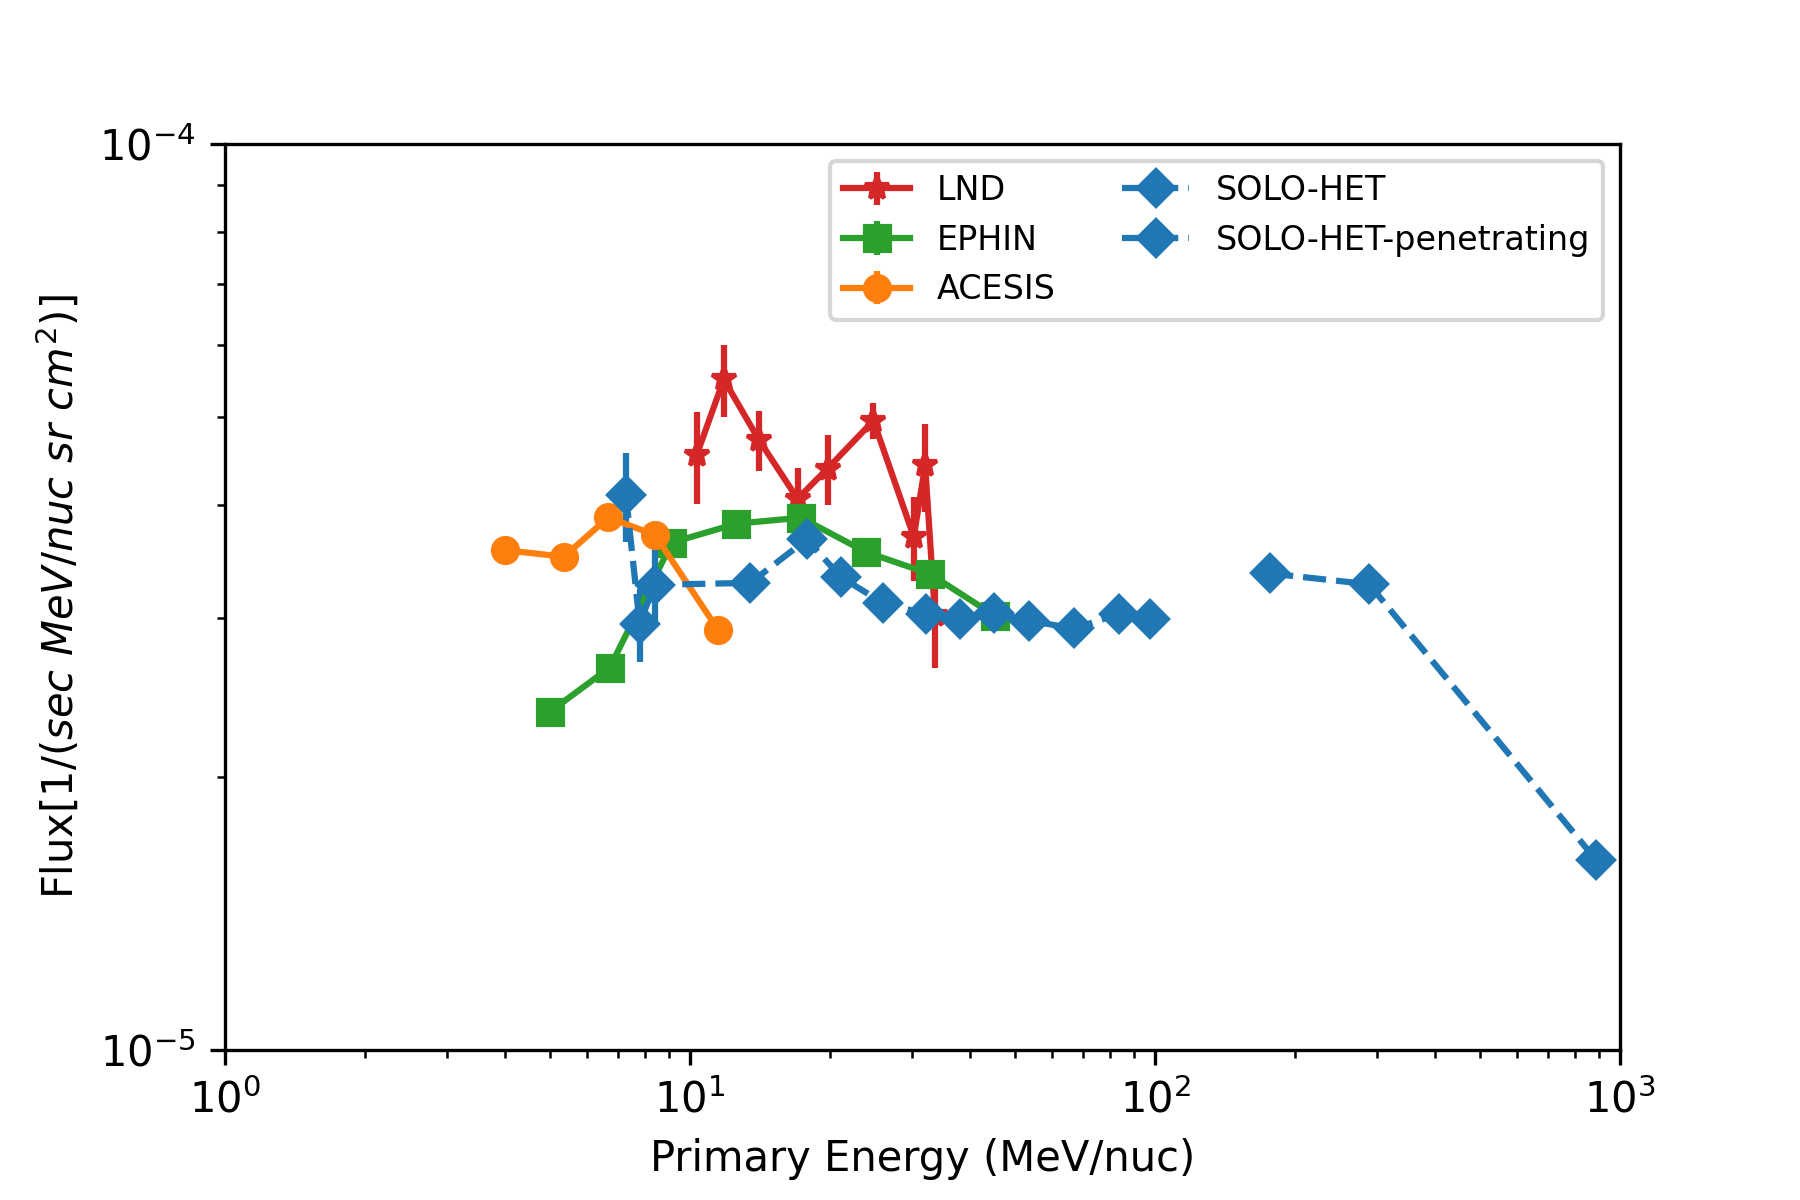
\includegraphics[width = 0.8\textwidth]{images/ACR/1AU_comparison_ACE_EPHIN_SOLO_SEP_version2.png}
    \caption[The helium spectra during the period \ac{SolO} between 0.95 and 1 au]{The helium-4 spectra of \ac{SolO}/\ac{HET}, \ac{SOHO}/\ac{EPHIN}, \ac{ACE}/\ac{ACESIS} and Chang'4/\ac{LND} when SOLO was between 0.95 and 1AU. The \ac{SEP} events are removed.}
    \label{fig:helium_spec_1au}
\end{figure}

\subsubsection{Two years' temperal variation of helium-4}

Fig.~\ref{fig:overview_helium_intensity} presents the intensity profile of helium on the reconstructed energy channels from \ac{HET}, \ac{EPHIN}, \ac{LND} and \ac{STEREO}-A. The energy range of recontructed channels are labeled in the legend correspondingly. The measurements are from Feb 2020 to October 2022. In the bottom panel, we again plot the orbit distance variation of \ac{SolO}.

It is evident from the observations that from 2020 to the middle of 2021, the measurements in the first half of period are generally dominated by the \ac{ACR} helium with only a few large \ac{SEP} events occuring at the end of 2020. After that with the increase of solar activities, the appear frequency of \ac{SEP} noticeably increase. Particularly, the solar energetic helium arrive differently at the \ac{SolO}, \ac{EPHIN} and \ac{STEREO}-A.
Those large and intense \ac{SEP} significantly disturbe the time profile of the \ac{ACR} background and consequently, we must remove them before calculating the \ac{ACR} radial gradient. Of note, the discoutinuity of \ac{LND} measurement are due to the hibernation of instrument during the lunar local night.

In addition to the intermittent occuring \ac{SEP}, the long-term decrease is also evident in the \ac{SolO} and \ac{EPHIN} measurements from 2020 to the end of 2022. This is because of the enhanced solar modulation of the solar magnetic field which is change with the solar cycle. The interplay between the large scale \ac{HMF} significantly reduce the number of \acp{ACR} arrival at the Earth and inner heliosphere below 1 au. We could foresee the further decrease of the \ac{ACR} intensity in the new few years before the solar acitivity reach the maximum in 2025 \citep{}.

In contrast to the transient variation from \ac{SEP} and 11-years variation due to the large scale solar modulation, the intensities of cosmic rays are also influenced and modulated by an recurring compressed structures that form from the interaction between fast and slow solar wind stream, emiting from the solar surface. Such a structure has enhanced pressure and density and occurs periodically with a period of approximately 27 days, i.e. the solar rotation period. This is so-called stream interaction region or corotating interaction regions \citep{Burlaga9174, Gosling1976, Schwenn1990, Richardson2004}. The changes of the local conditions modify the transport of cosmic rays and the consequence reflects on the intensity changes, though such variation is not as significant as the \acp{SEP} and solar modulations.

\begin{figure}
    \centering
    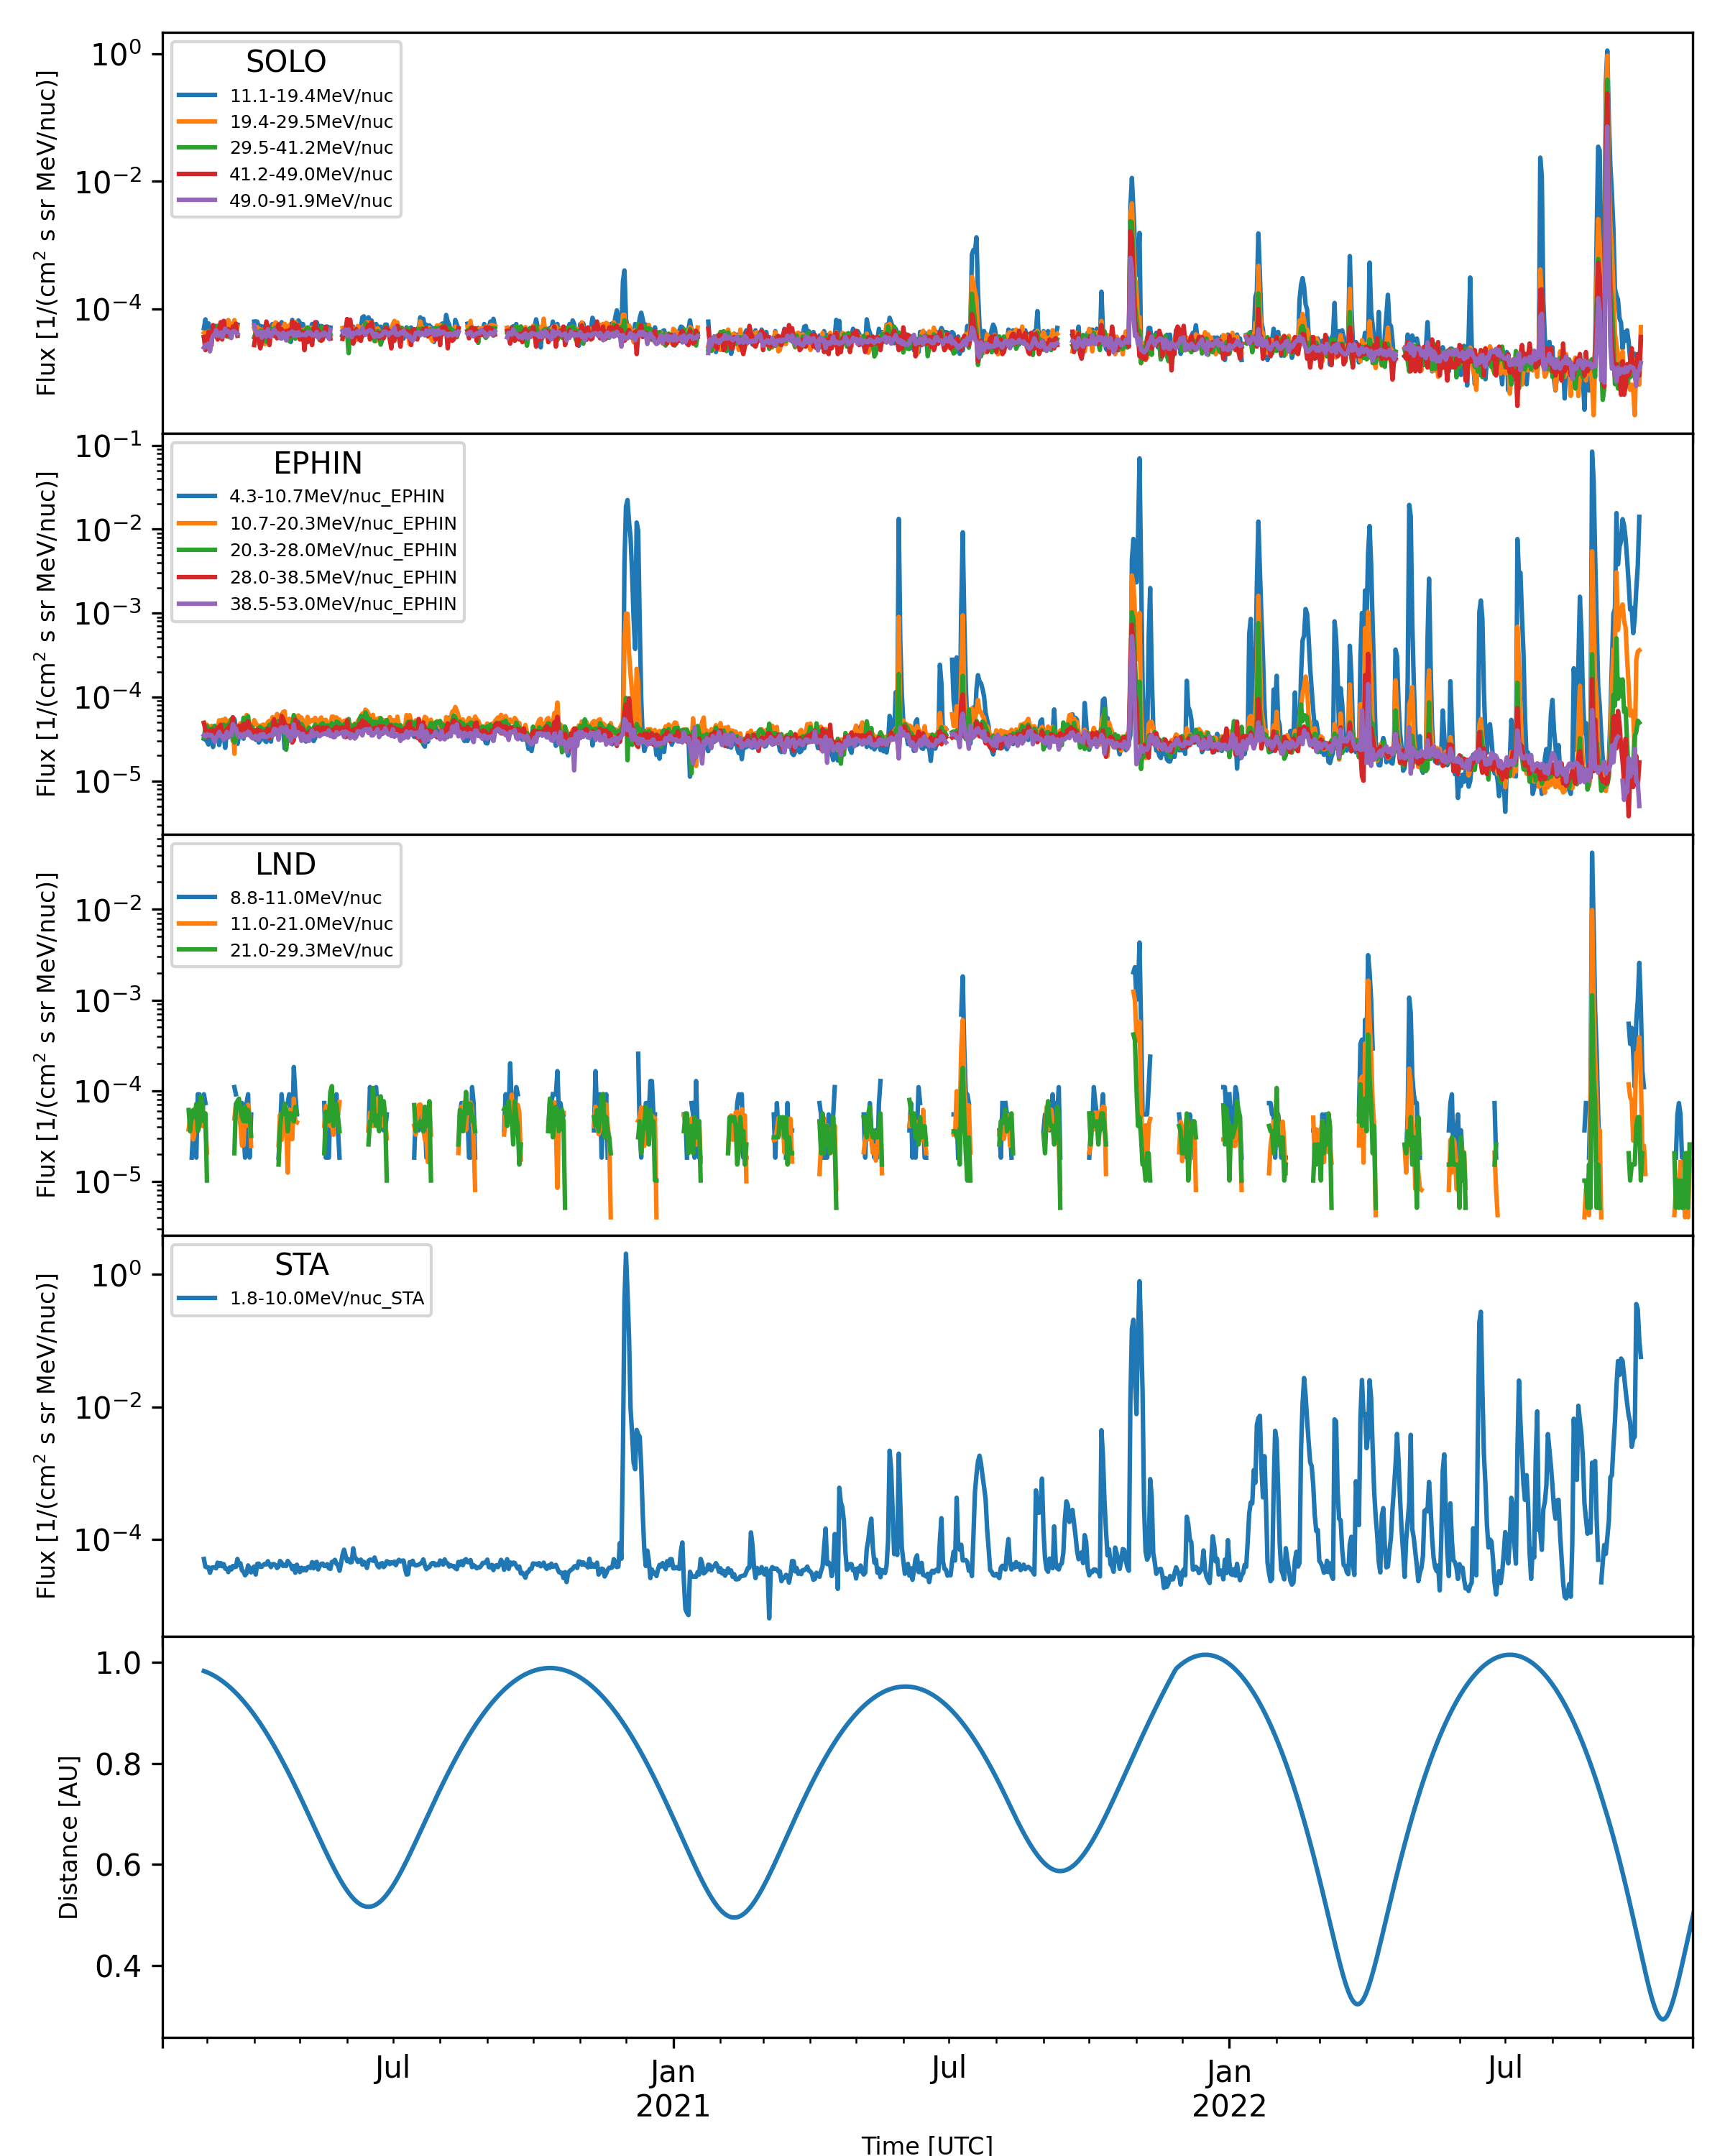
\includegraphics[width = 0.8\textwidth]{images/ACR/overview_Helium_4_instrument.png}
    \caption[Overview of the helium measuremet by different instruments]{From top to the bottom: The daily averaged helium flux measured by \ac{SolO}/\ac{HET}, \ac{SOHO}/\ac{EPHIN}, Chang'E-4/\ac{LND}, and \ac{STEREO}-A/\ac{LET} over 2020.2 - 2022.10. The bottom plot shows the radial distance of \ac{SolO} away the sun.
    %The red dashed lines indicate the SEP events that we determined by eye.
    \TODO{reminder: you should better re-load the SOLO data, and check the isotropic between different direction, and resample data before further process like sum all direciton or somesome.}}
    \label{fig:overview_helium_intensity}
\end{figure}




\begin{table}[]
    \centering
	\caption[Time perods \ac{SolO} closed to 1 au]{A list of time perods when the solar radial distance of \ac{SolO} is between 0.95 and 1 AU. The distance between \ac{SolO} and Earth is also given.}
	\label{tab:1AU_period}
    \begin{tabular}{|c|c|c|c|}
    \hline
	periods & start time & end time & distance to Earth  (au)\\
    \hline
    1   & 2020-02-28 & 2020-03-16   & 0.07 \\
    \hline
	1	& 2020-09-14 & 2020-11-10	& 1.76 \\
    \hline
	2	& 2021-05-27 & 2021-06-09	& 1.49 \\
    \hline
	3	& 2021-11-21 & 2022-01-15	& 0.13 \\
    \hline
	4	& 2022-06-05 & 2022-08-02	& 1.96 \\
    \hline
    5 (not used)	& 2023-01-04 & 2023-01-17	& 0.41 \\
    \hline
    \end{tabular}
\end{table}


\subsection{\ac{SEP} list}

As we aforementioned, the \acp{SEP} is one of most manifest disturbance to the \ac{ACR} background. Therefore, a completed and properly defined \ac{SEP} periods are crucial. In this section we explain what type of data we used and how we determine the \ac{SEP} periods.

The \ac{SEP} arrived differently at \ac{SolO} and at the Earth. Hence, the \ac{SEP} list are determined seperated for both cases.
Moreover, in order to remove the solar particle thoroughly and prevent the existence of remanent particles that could not be recognized directly from the intensity profiles, we consider utilizing different measurements to identify the \acp{SEP}.

Fig.~\ref{Fig:solo-lvl2} presents the 10 minute count rate of L2 counter named HET_any(a1, b1) and HET_any(a2, b2). As we explained in the instrument section, those channels are perfect indicator of the \ac{SEP} with larger counting statistics, approximately 600 counts per ten minutes. The \ac{SEP} list at Earth is determined by the time profile of lower energy proton below 10 MeV that observed from \ac{EPHIN}.

The duration of the SEP is simply determined by the 3-$\sigma$ method with the eye determination as supplements. $\sigma$ is the standard deviation of a background or the preevent quite time. The \ac{SEP} periods are defined as the consecutive time series when the flux is 3 time of the standard derivations above the background. This method was commonly used in determining the onset time of the SEPs event and valid for those SEPs has clear onset and sharp increase. 
However, if the background is unclear and increase of the temporal profiles is slow, the determination of the onset and end of event might have larger uncertainty. In this case, we determine the boundary of periods by eye.

As a result, the \ac{SEP} periods that we determined are illustrated as the magenta color region in Fig.~\ref{Fig:solo-lvl2} and Fig.~\ref{Fig:SOHO_EPHIN_Proton_flux} and  the \ac{SEP} priods are listed in Table.~\ref{tab:SEP_list} in Appendix.



\begin{figure}
    \centering
    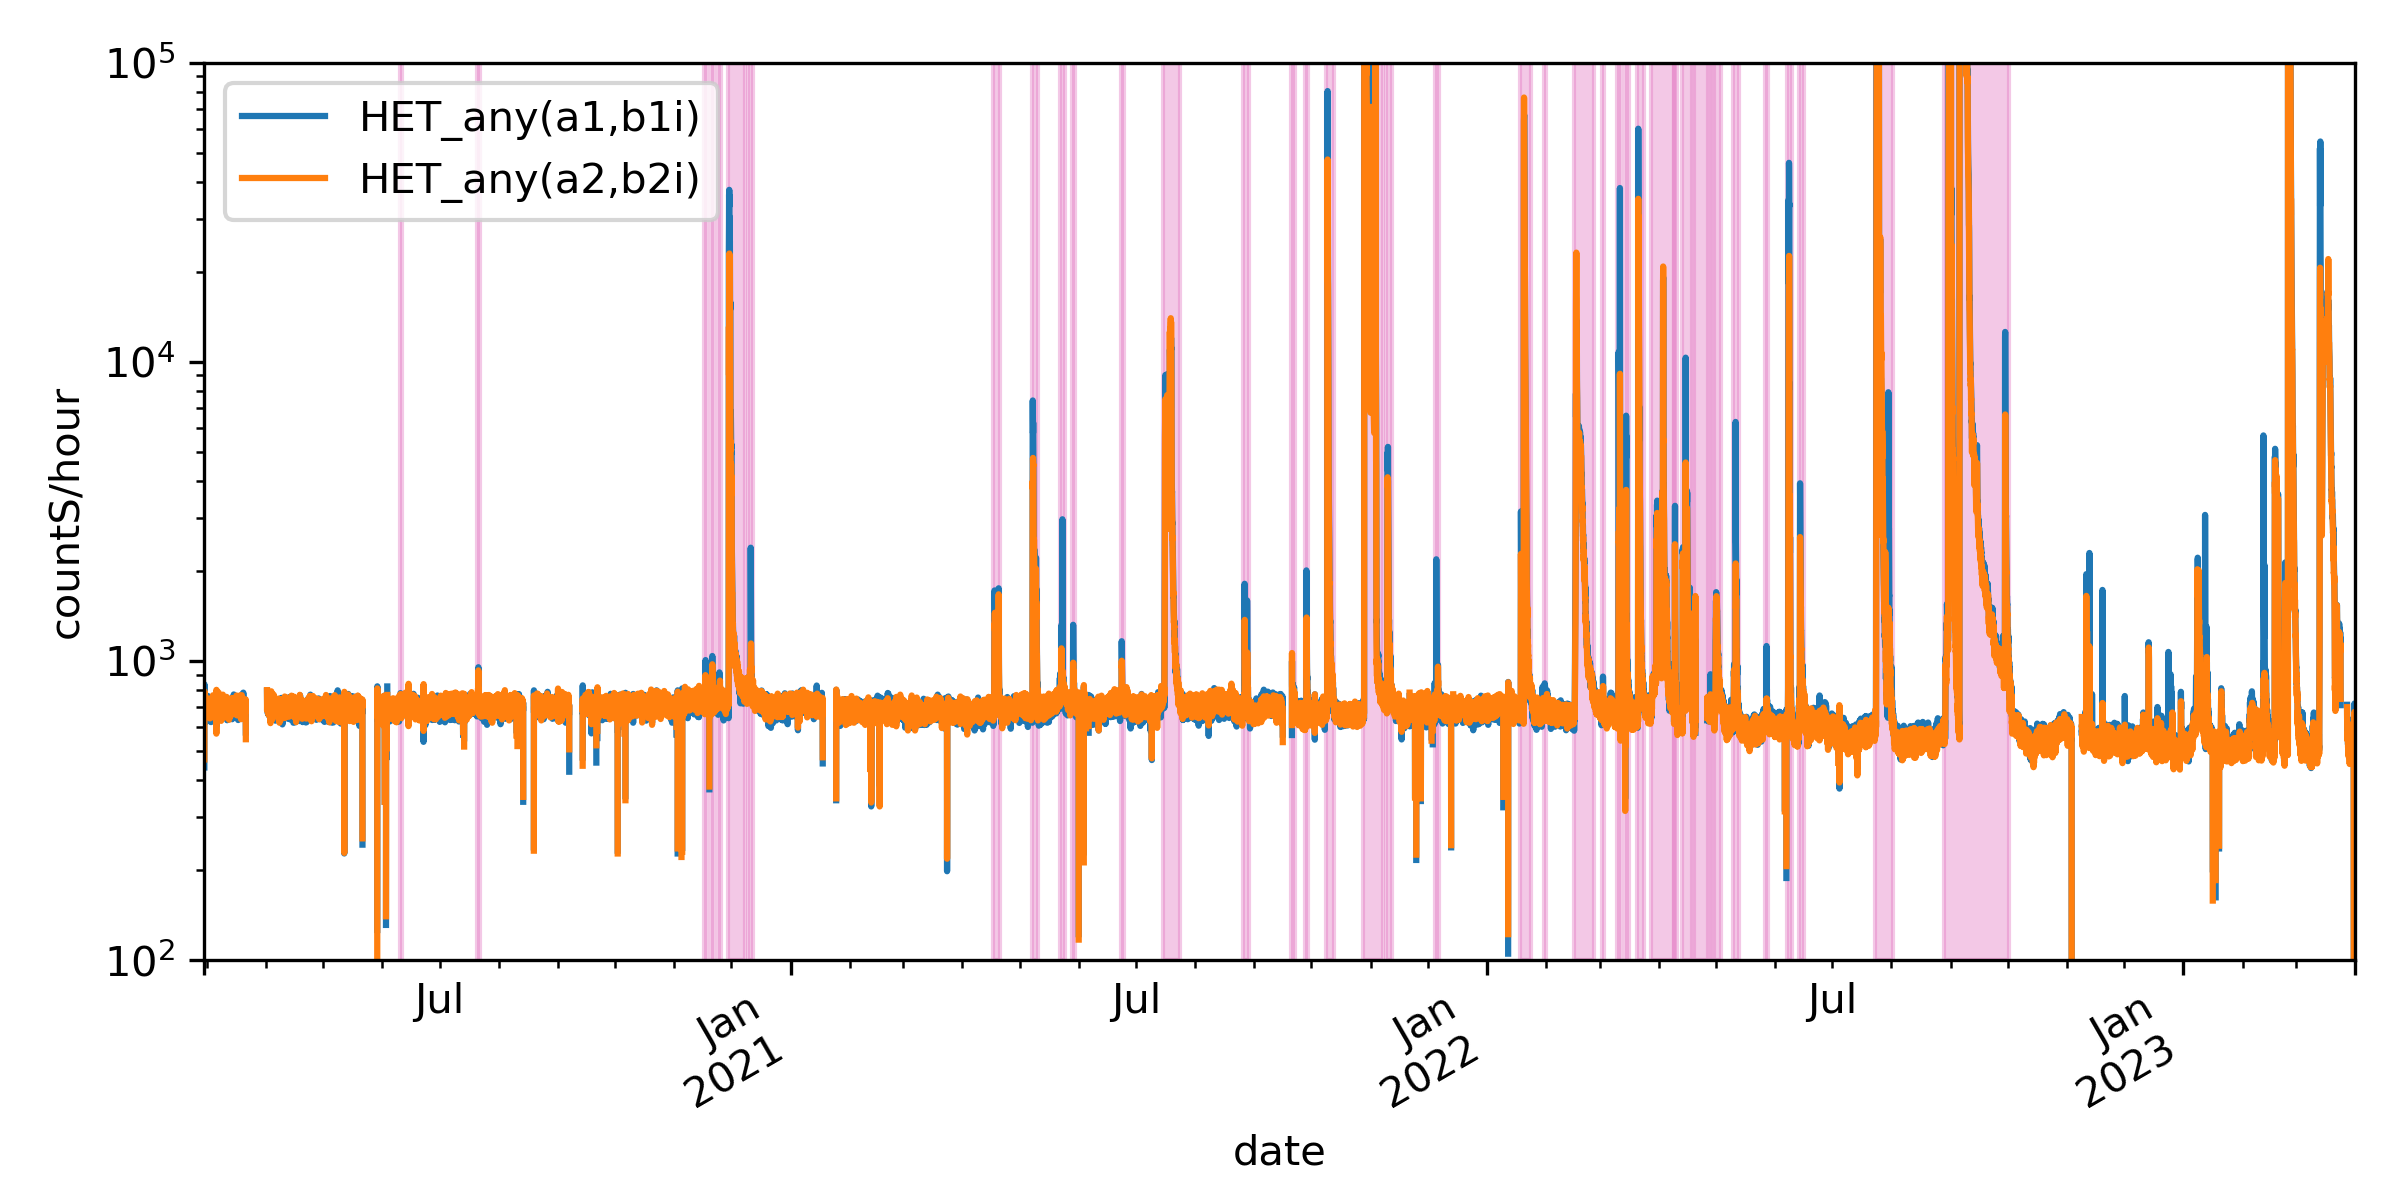
\includegraphics[width = \textwidth]{images/ACR/SOLO-lvl2-trriger.png}
    \caption{The Level-2 counter of the \ac{HET} named any(a1,b1) and any(a2,b2). The magenta color regions are the SEP periods we identified.}
    \label{Fig:solo-lvl2}
\end{figure}



\begin{figure}
    \centering
    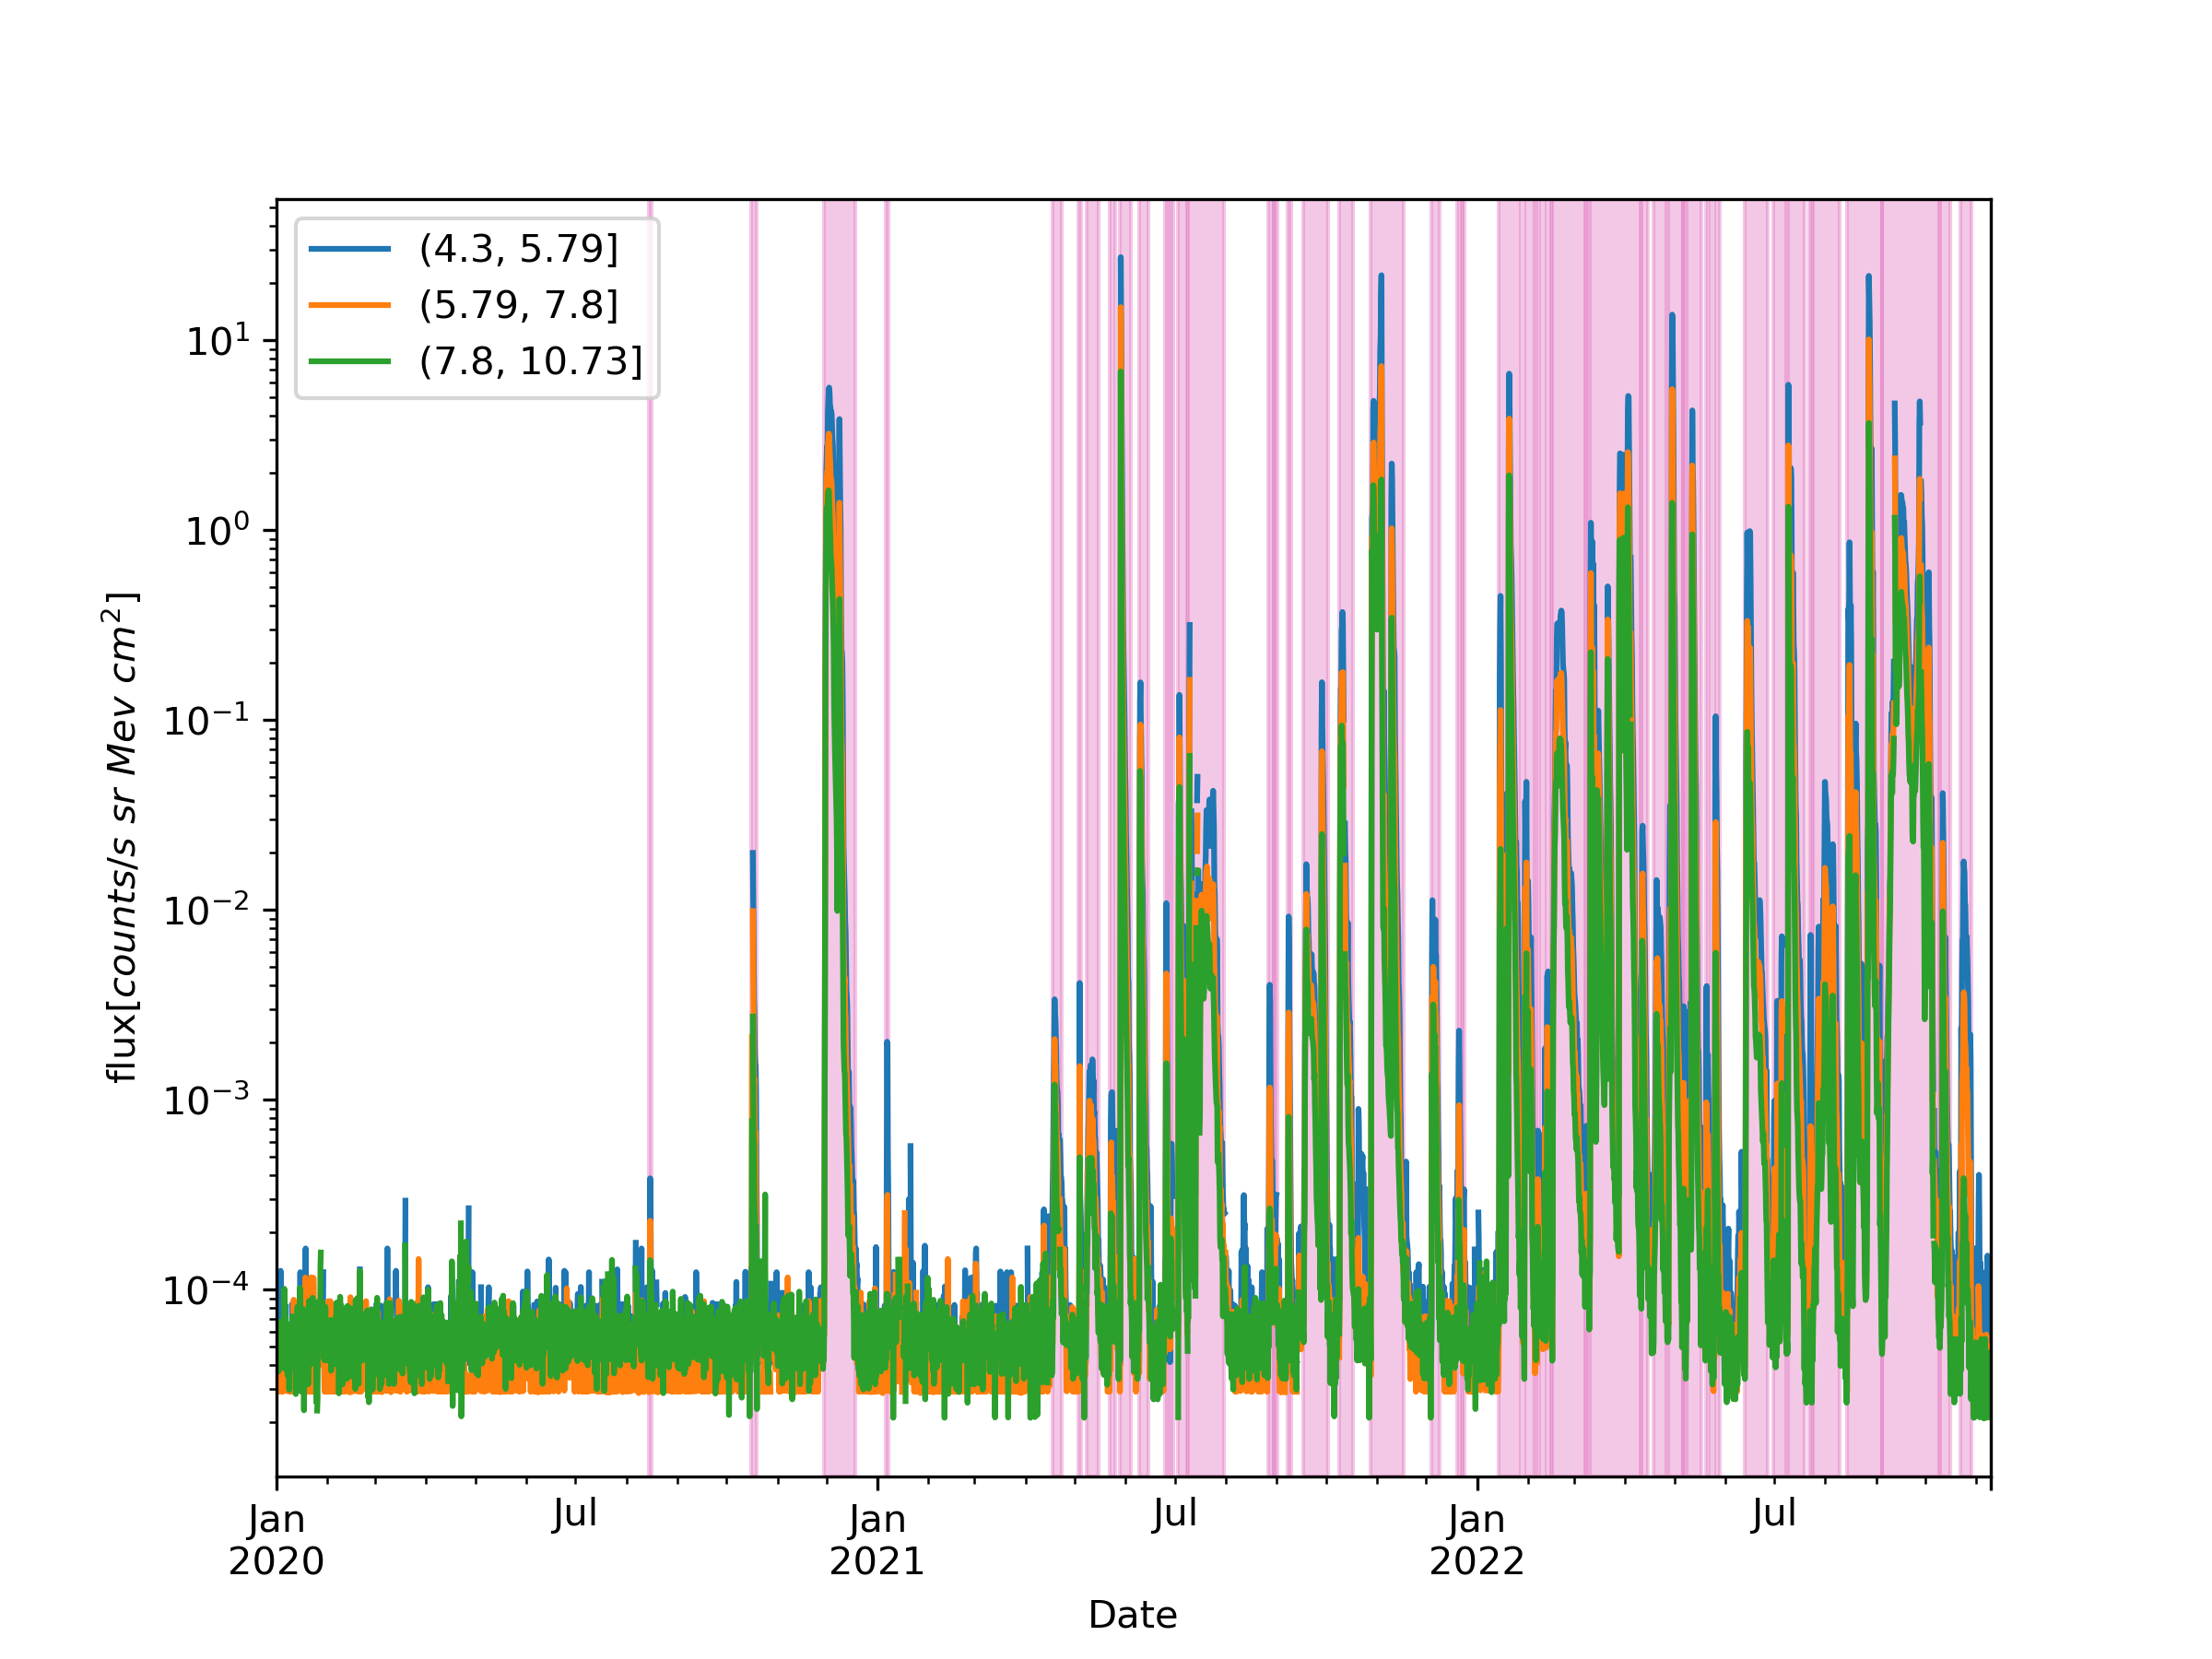
\includegraphics[width = 0.8\textwidth]{images/ACR/SOLO-EPHIN-l3i-log2+6-proton-6H.png}
    \caption{The proton flux measured by SOHO/EPHIN below 10 MeV. The data we used here are the level-3 proton data products. The magenta shadow regions are the SEP.}
    \label{Fig:SOHO_EPHIN_Proton_flux}
\end{figure}

\subsection{Averaged over carrington rotation}

\begin{figure}
    \centering
    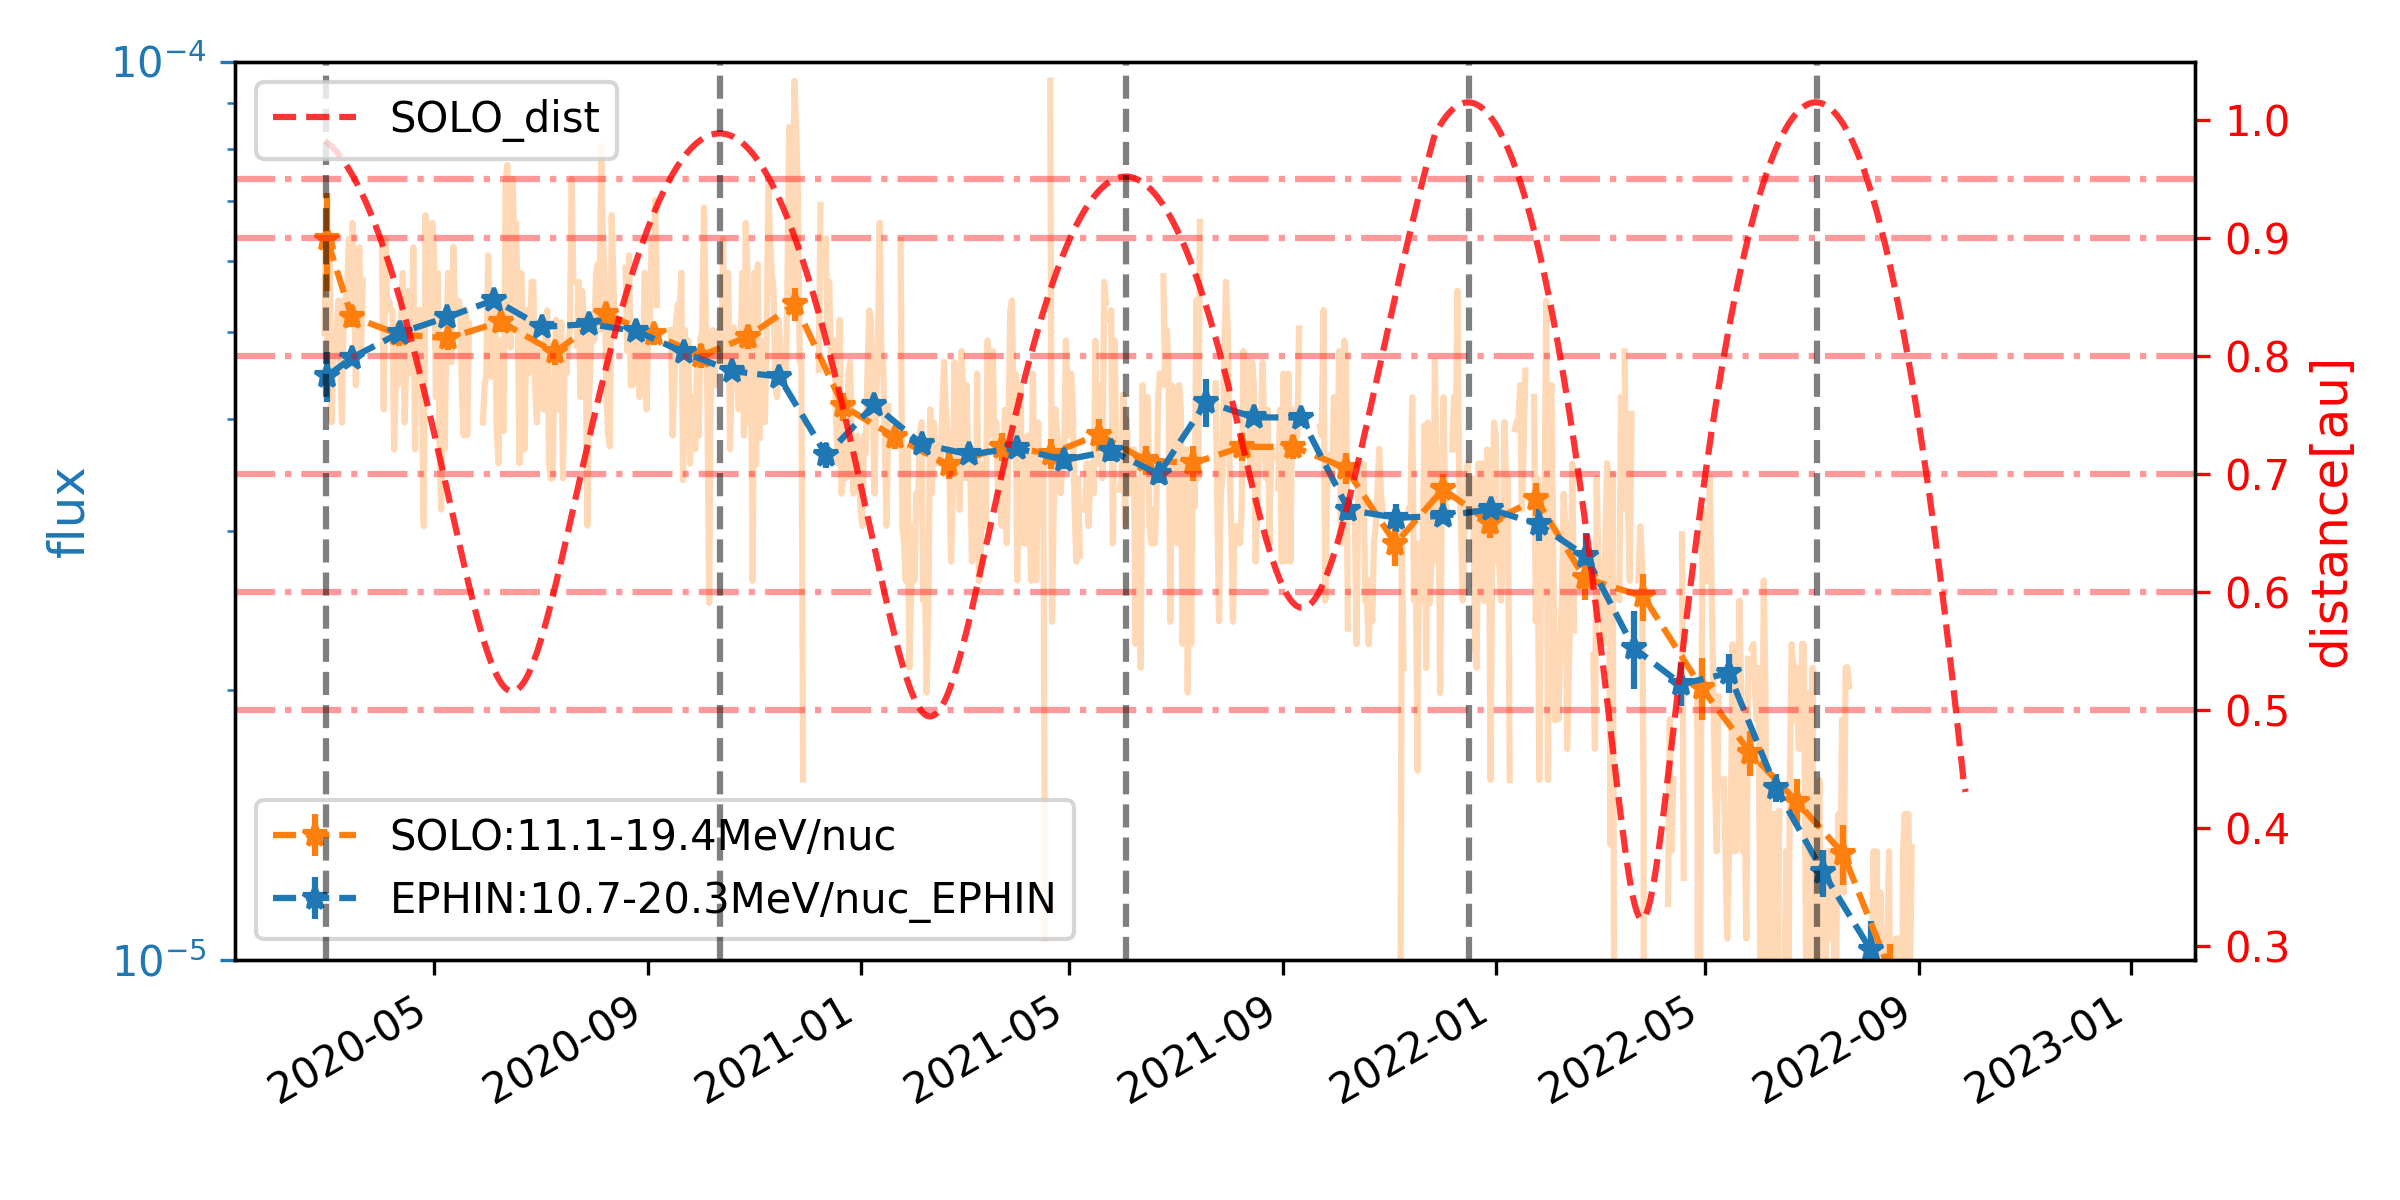
\includegraphics[width = 0.8\textwidth, height = 0.2\textheight]{images/ACR/seperate_mask_1-3/Carrington_SOLO_11.1-19.4MeV_EPHIN_10.7-20.3MeV.png}
    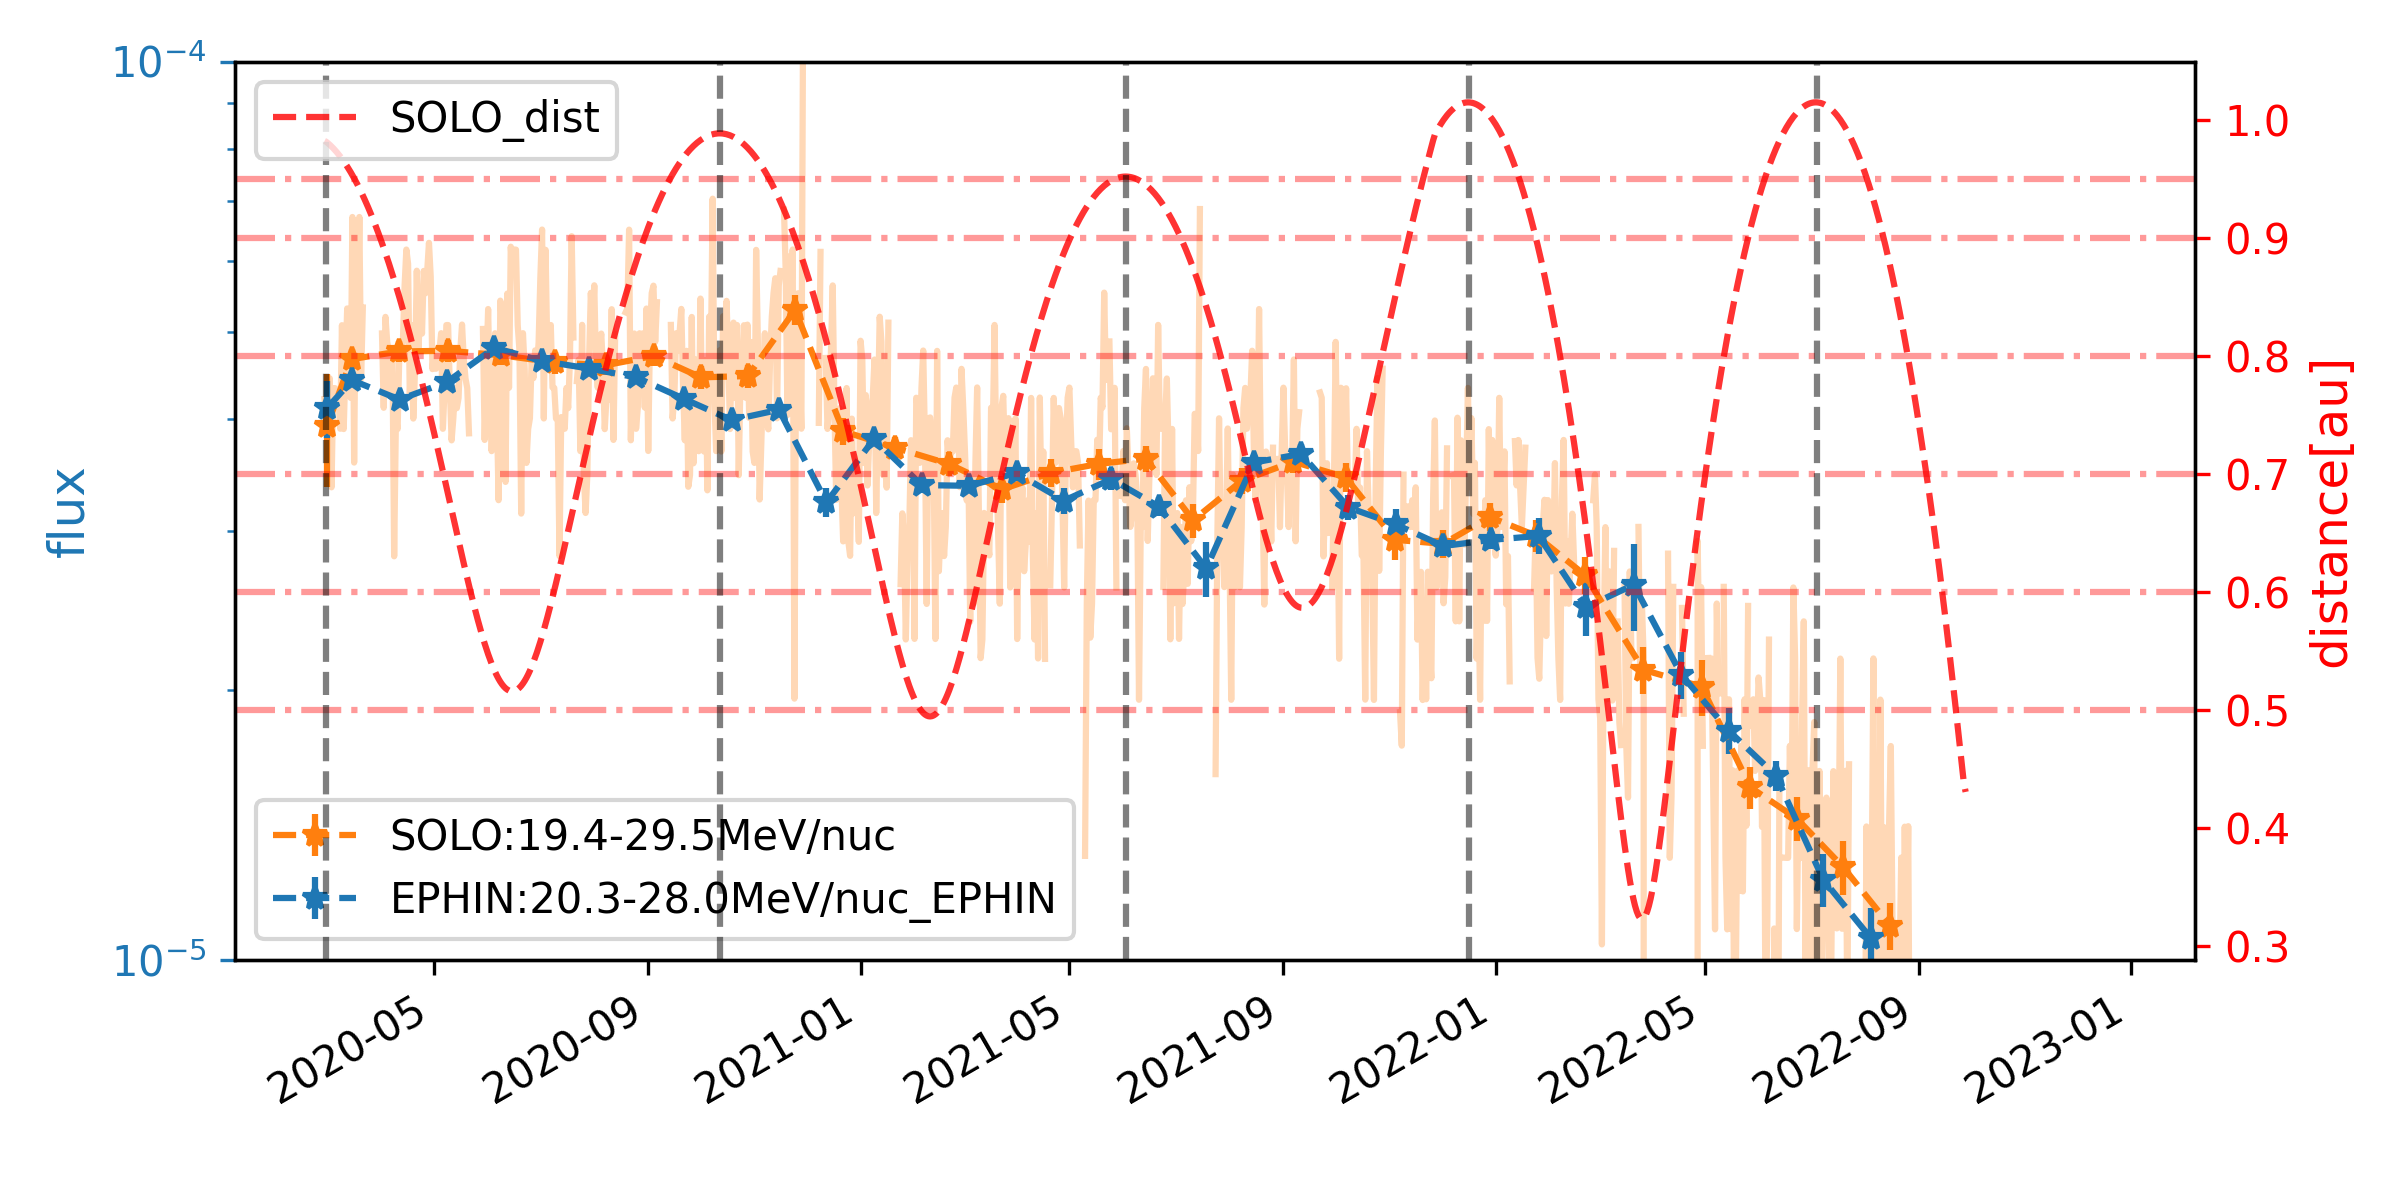
\includegraphics[width = 0.8\textwidth,height = 0.2\textheight]{images/ACR/seperate_mask_1-3/Carrington_SOLO_19.4-29.5MeV_EPHIN_20.3-28.0MeV.png}
    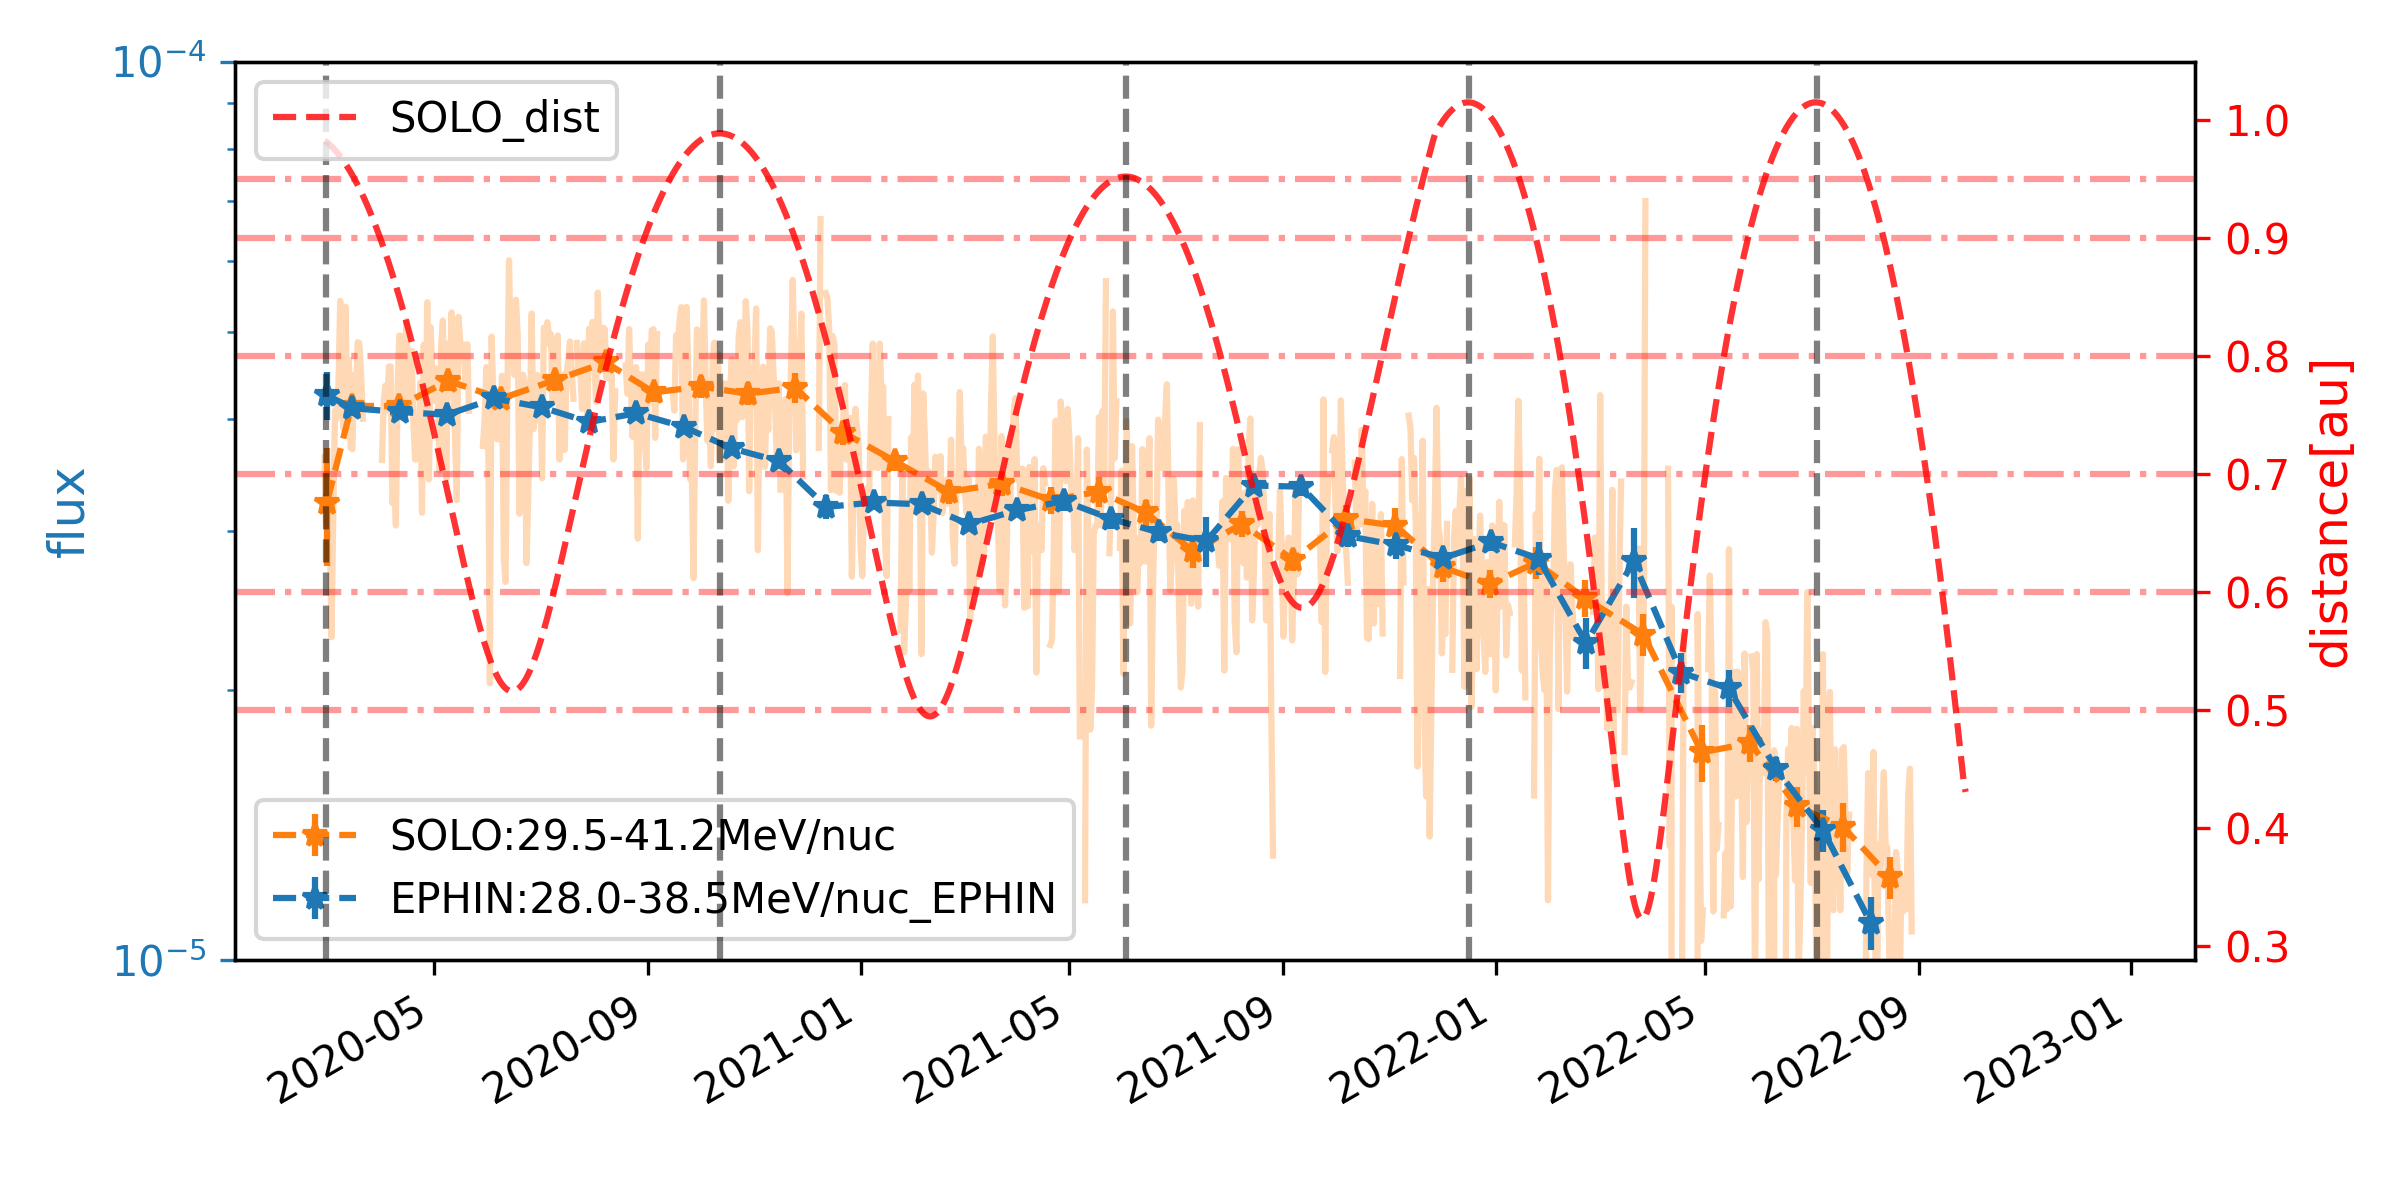
\includegraphics[width = 0.8\textwidth,height = 0.2\textheight]{images/ACR/seperate_mask_1-3/Carrington_SOLO_29.5-41.2MeV_EPHIN_28.0-38.5MeV.png}
    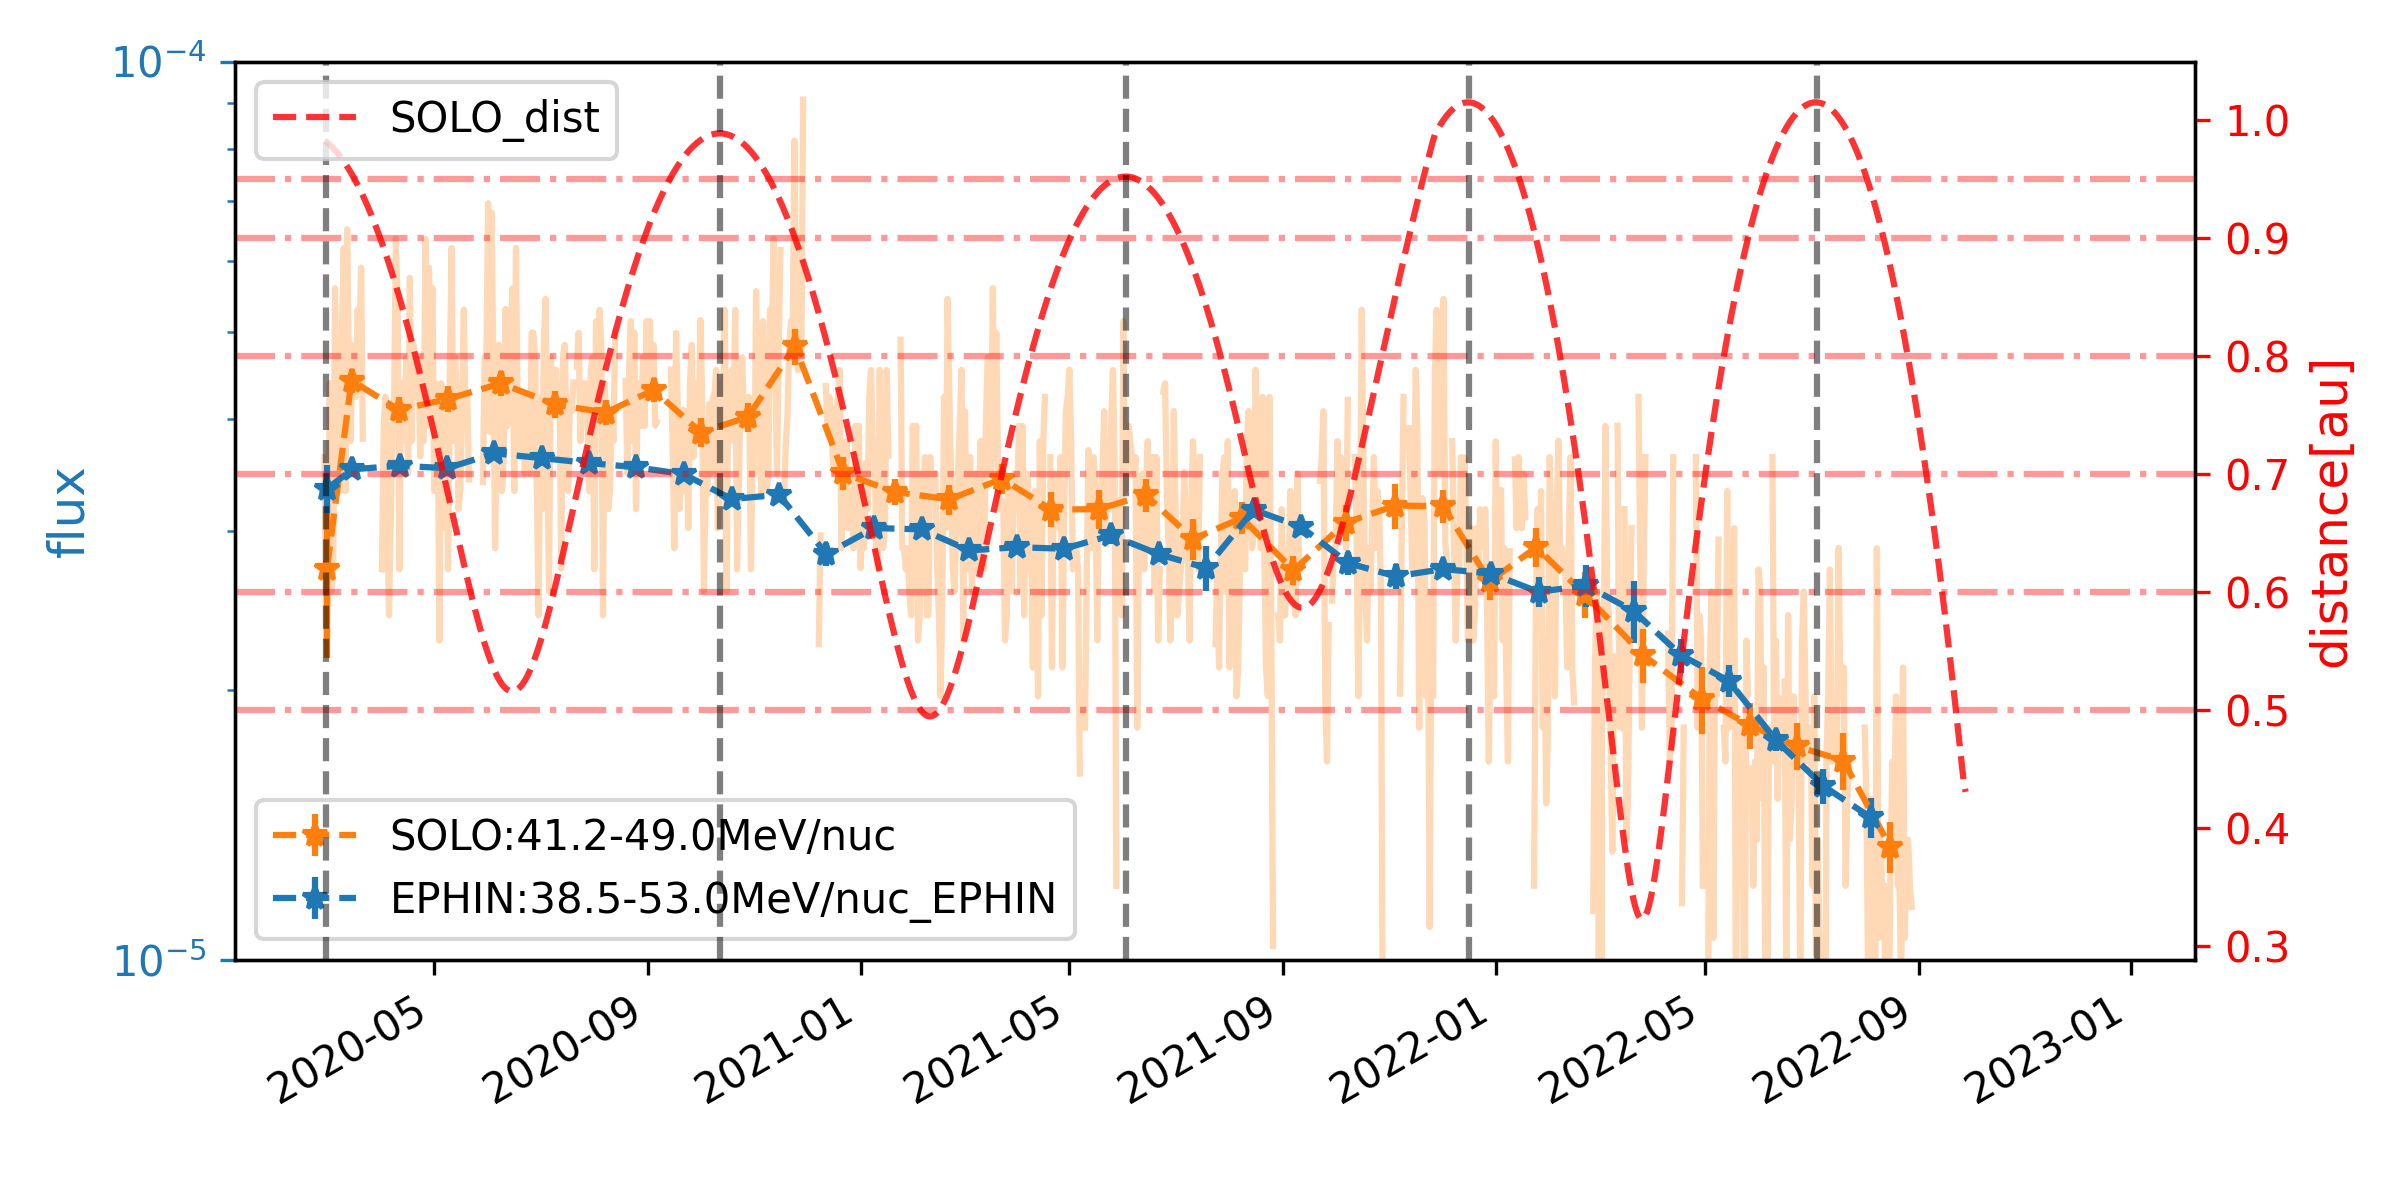
\includegraphics[width = 0.8\textwidth,height = 0.2\textheight]{images/ACR/seperate_mask_1-3/Carrington_SOLO_41.2-49.0MeV_EPHIN_38.5-53.0MeV.png}
    \caption{The carrington rotation averaged flux of SOLO (orange) and EPHIN (blue) in corresponding cordinate. The time profile in light orange color is the daily averaged SOLO/HET in different energy channel.}
    \label{fig:carrington_flux}
\end{figure}

\begin{figure}
    \centering
    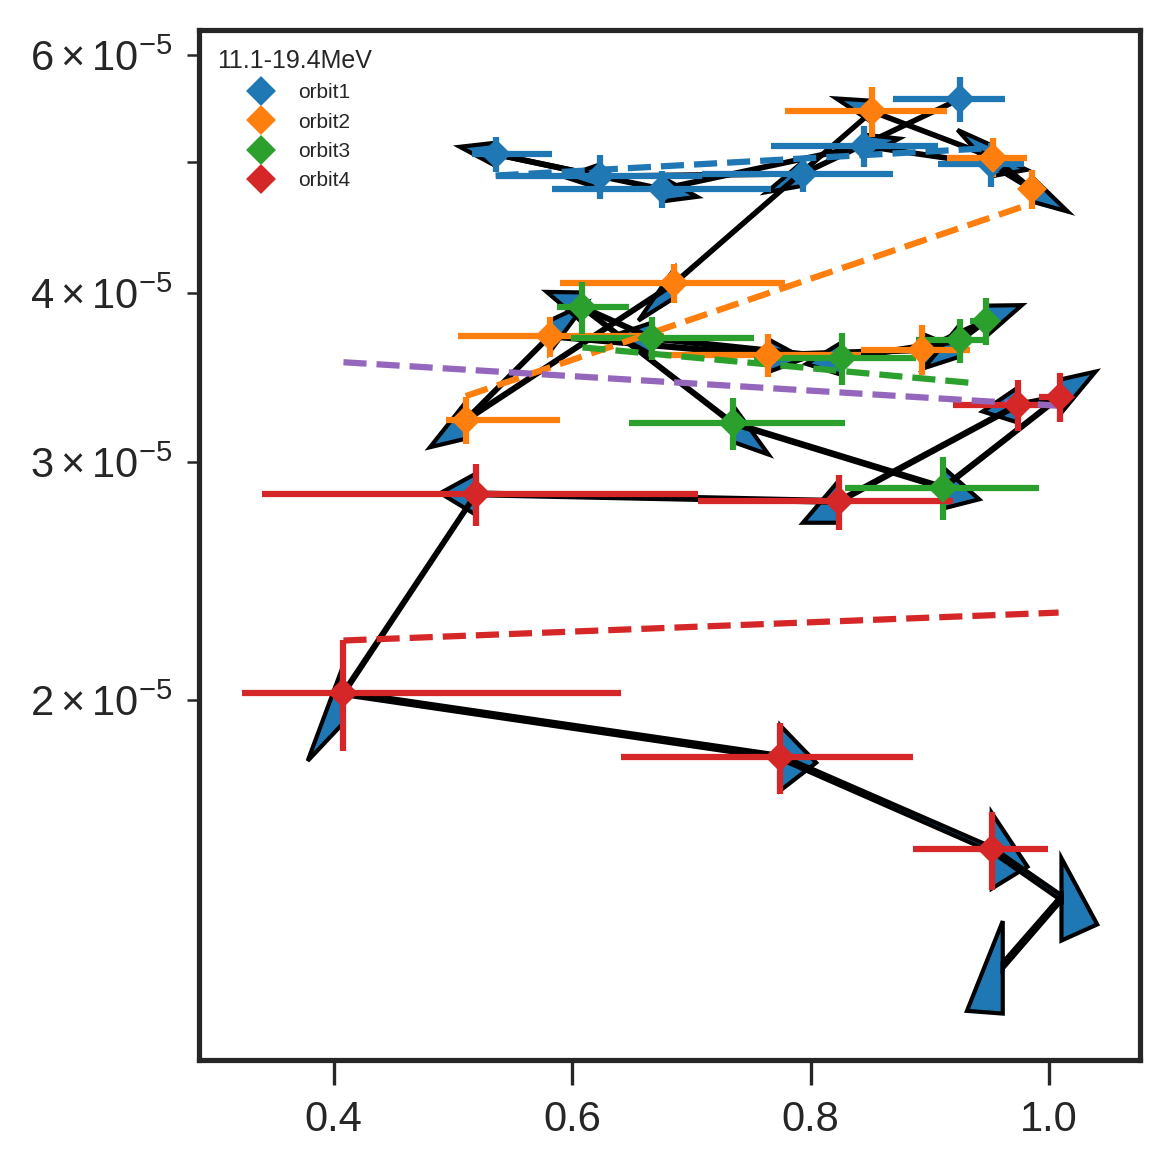
\includegraphics{images/ACR/SOLO-flux_only.png}
    \caption{The flux vs the radial distance of SOLO.}
    \label{fig:fluxvsdistance}  
\end{figure}


\subsection{Ratio of SOLO and EPHIN and radial gradient}

\begin{figure}
    \centering
    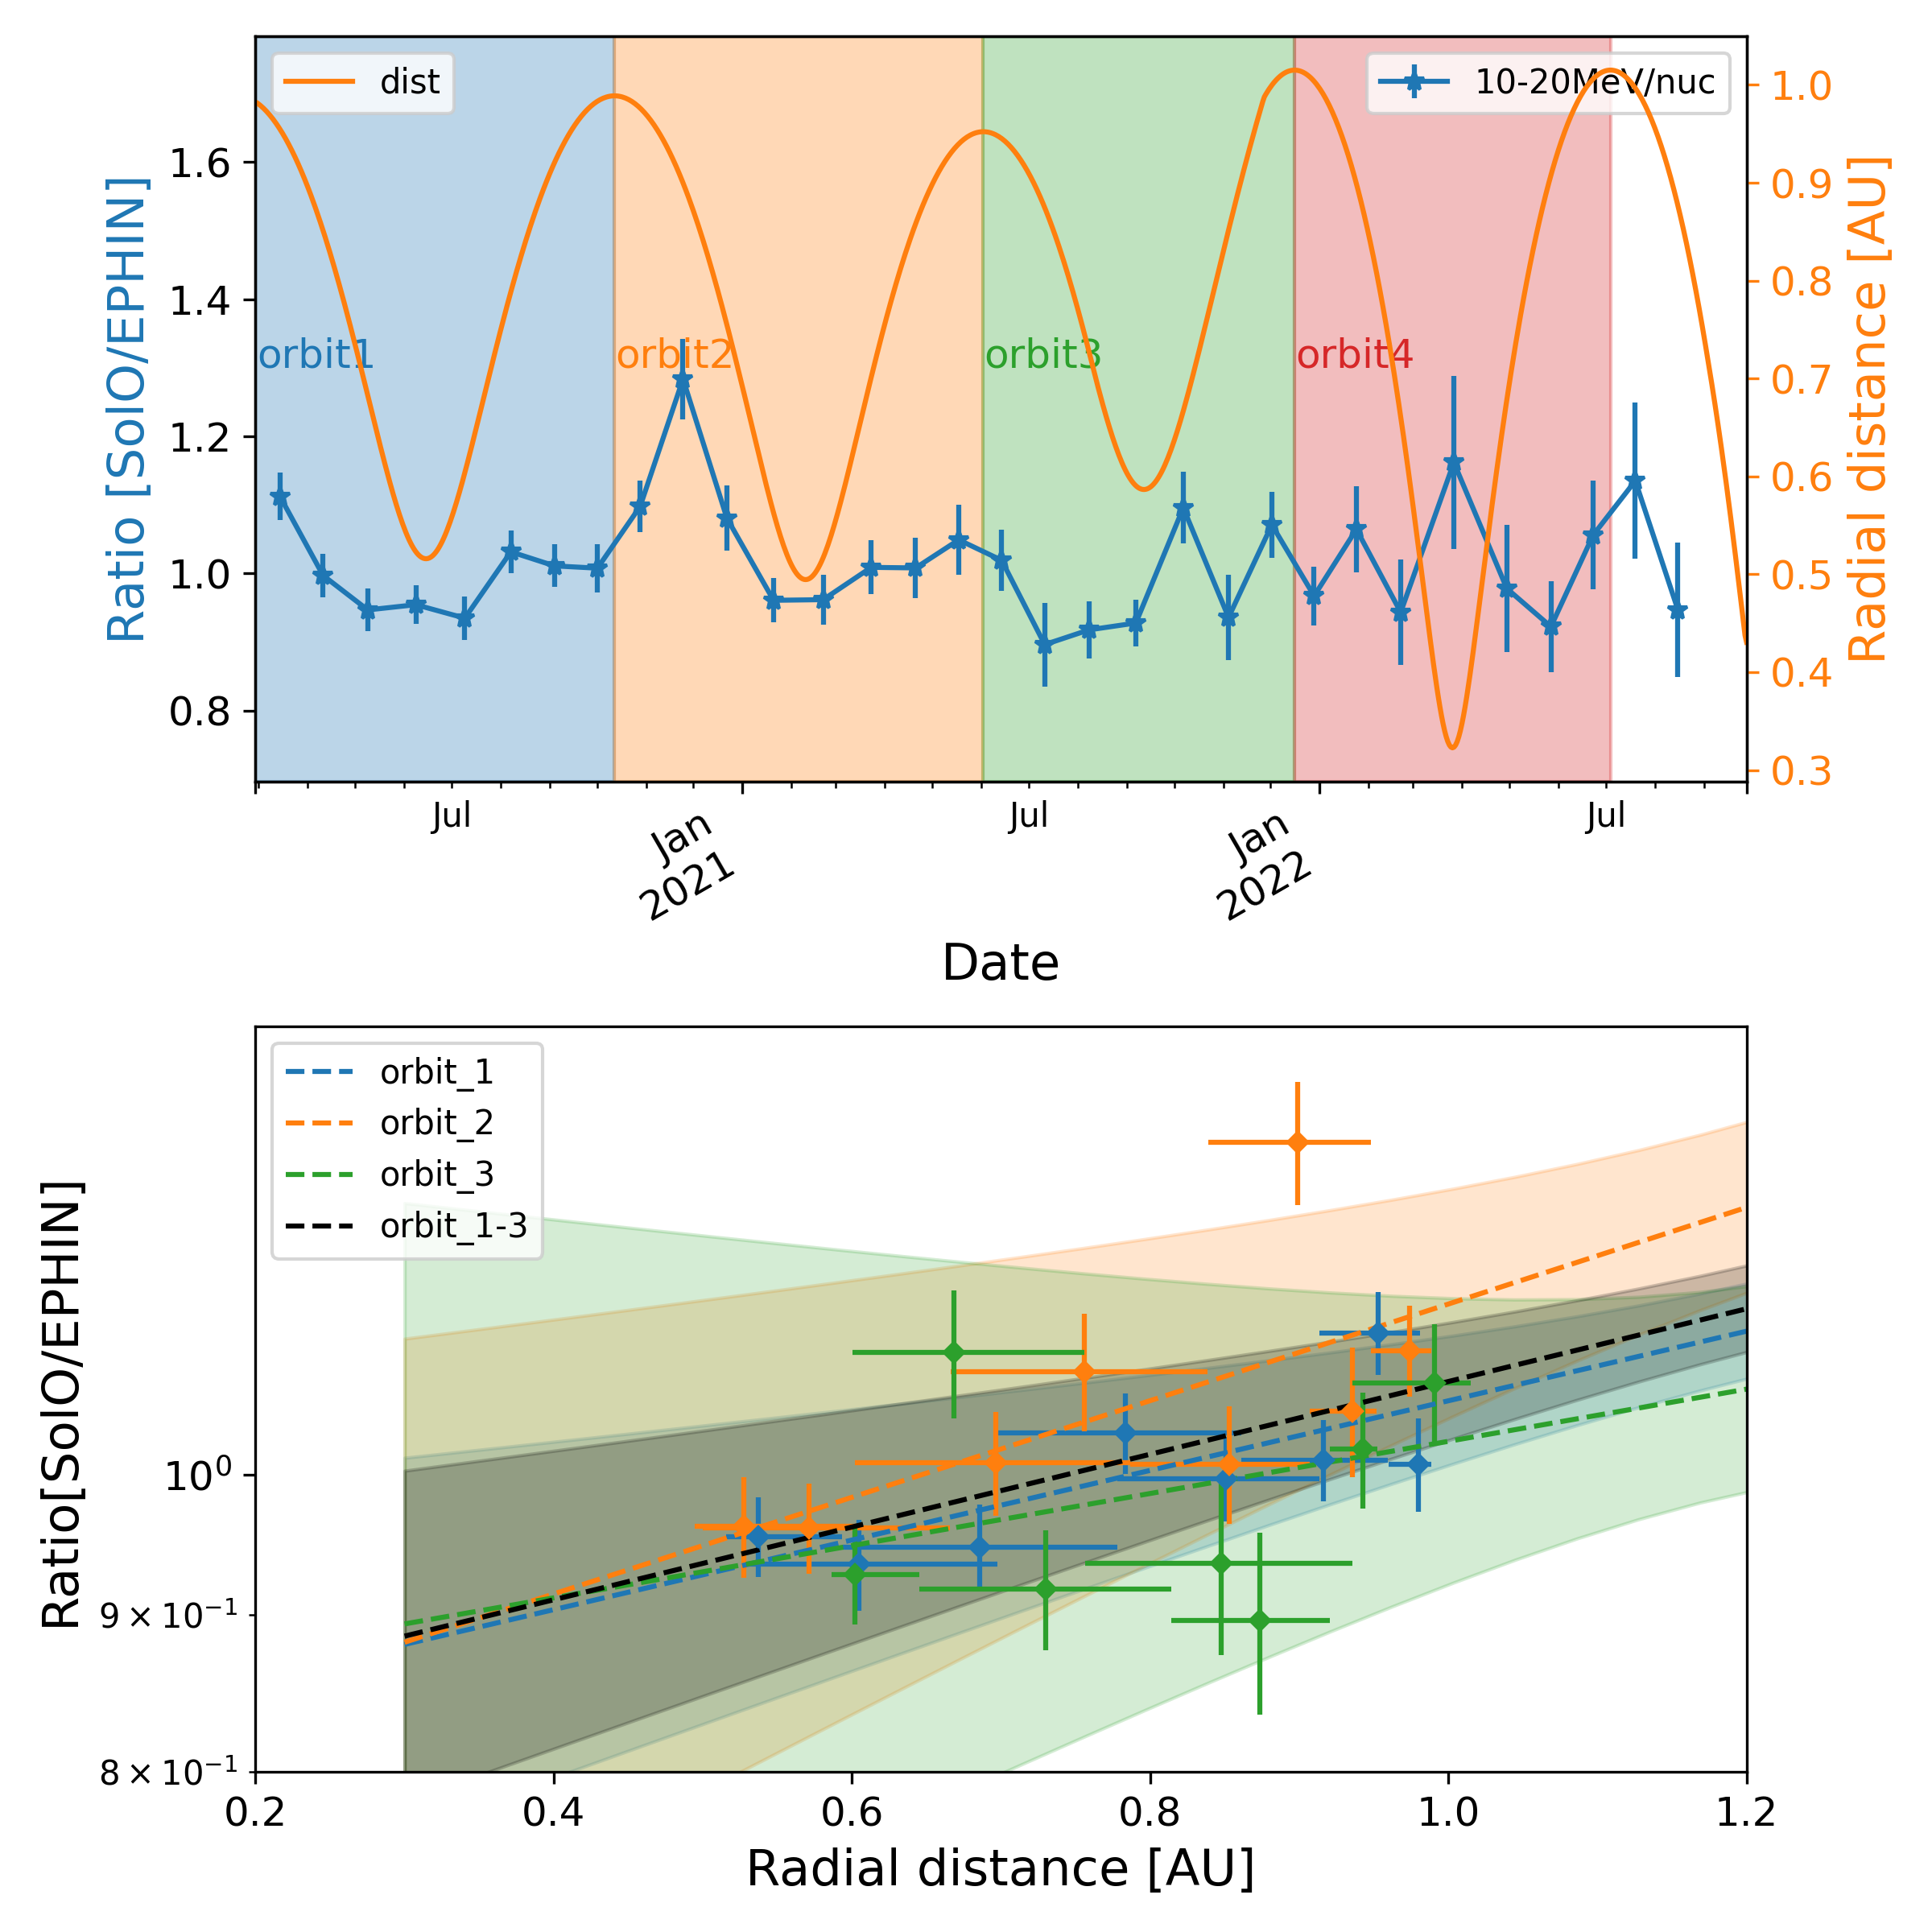
\includegraphics[width =0.4\textwidth]{images/ACR/seperate_mask_1-3/ratio_time_radialgradient_10-20MeV.png}
    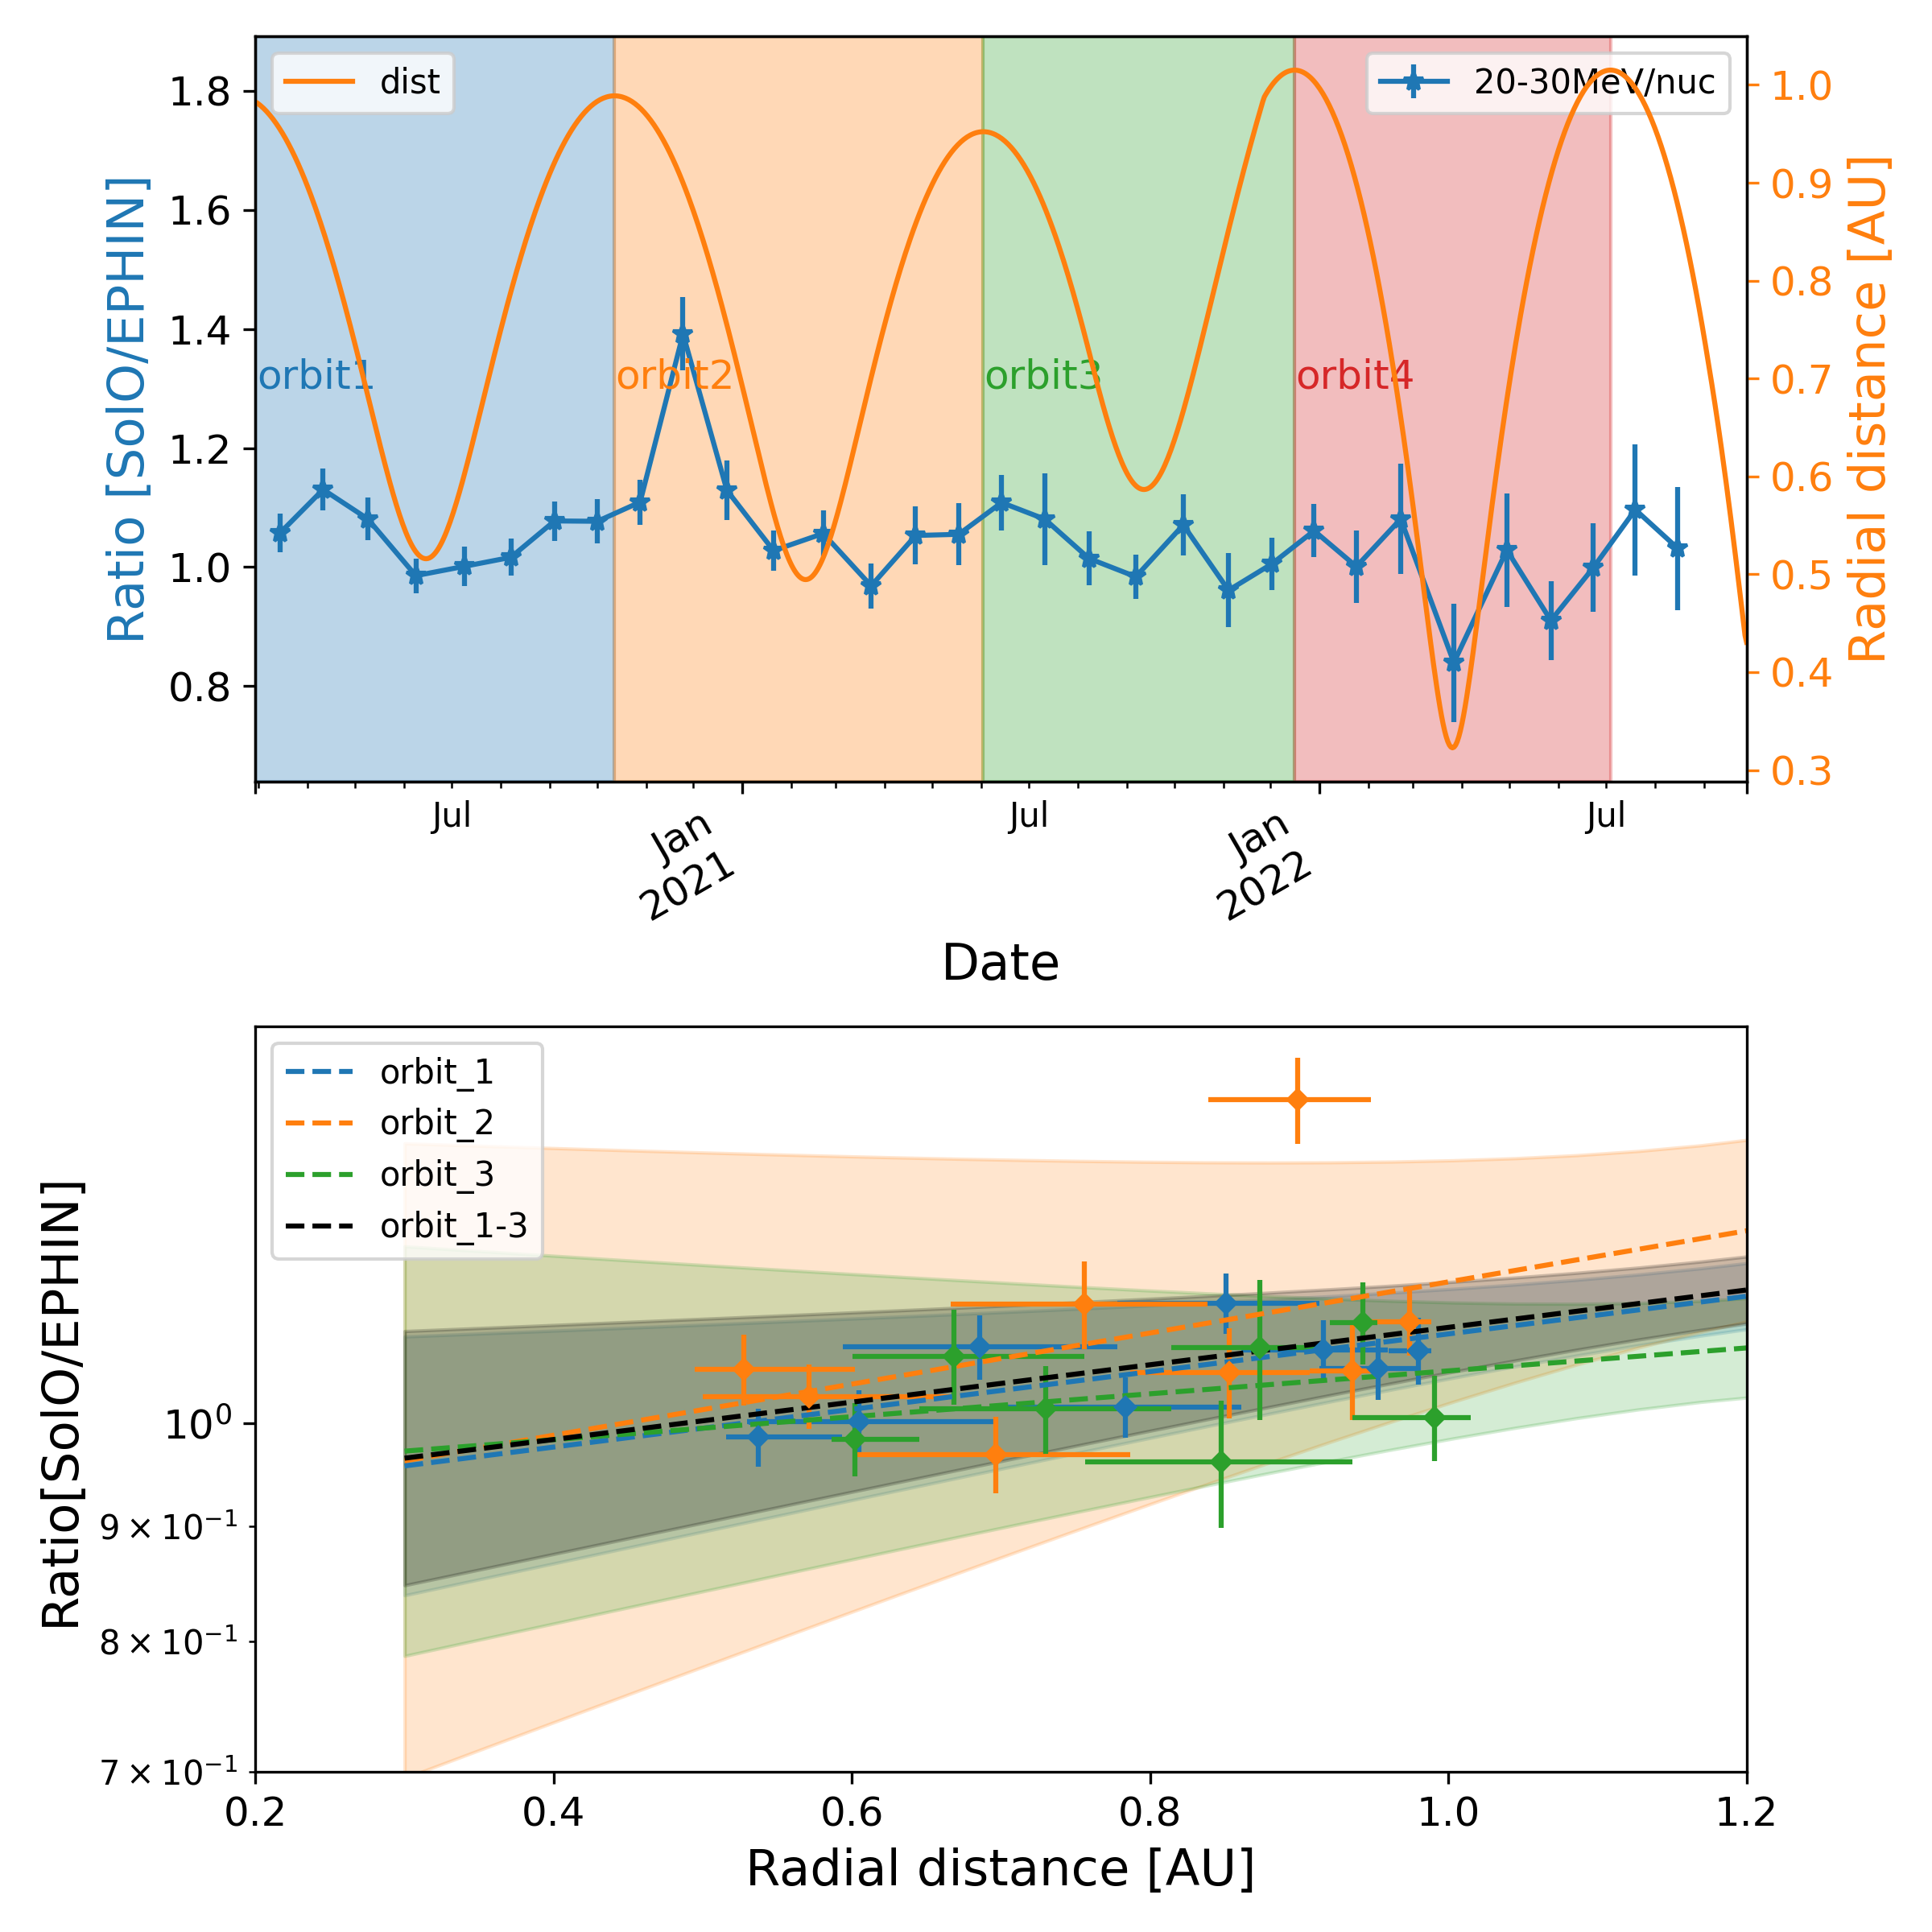
\includegraphics[width =0.4\textwidth]{images/ACR/seperate_mask_1-3/ratio_time_radialgradient_20-30MeV.png}
    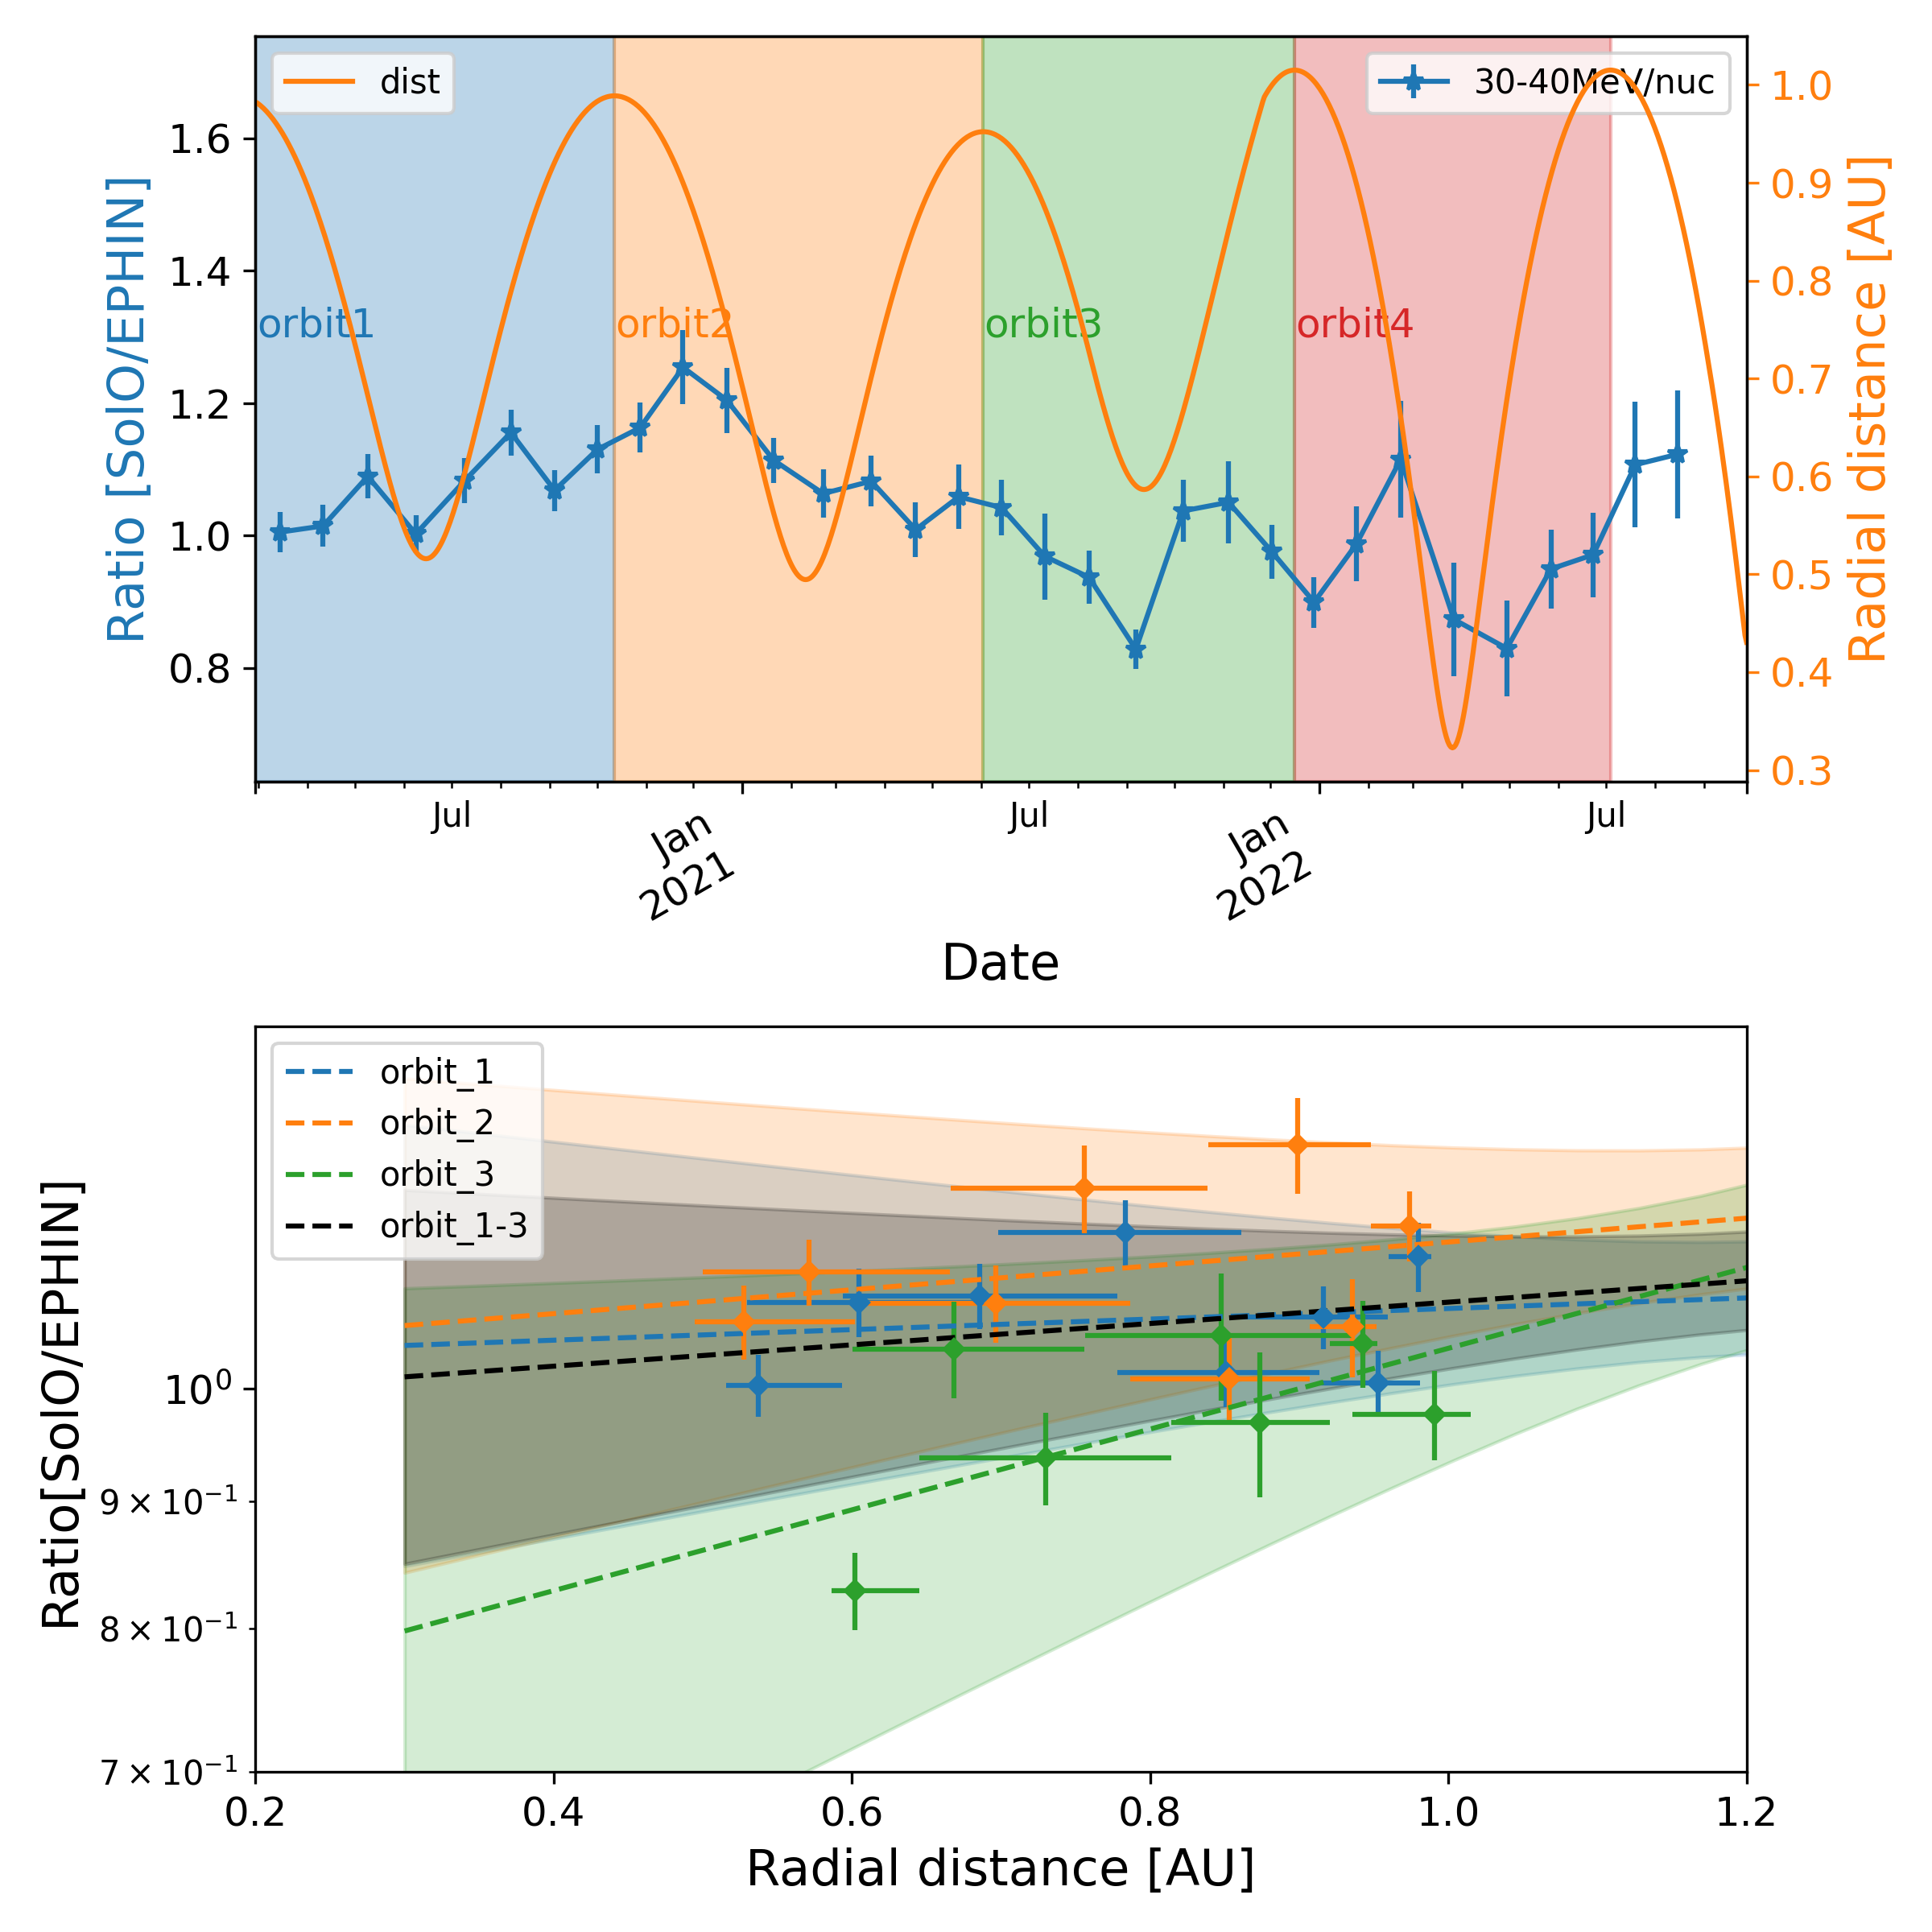
\includegraphics[width =0.4\textwidth]{images/ACR/seperate_mask_1-3/ratio_time_radialgradient_30-40MeV.png}
    \includegraphics[width =0.4\textwidth]{images/ACR/seperate_mask_1-3/ratio_time_radialgradient_40-50MeV.png}
    \caption{The ratio of SOLO and EPHIN in different energy channel changes over times. The ratio is calculated using the carrington averaged flux. The bottom panels of four subplots are the ratio vs the radial gradient. The data points in different colors are from different orbit as given in the legend.} 

\end{figure}

\subsection{Compared with model and the observations}
\begin{figure}
    \centering
    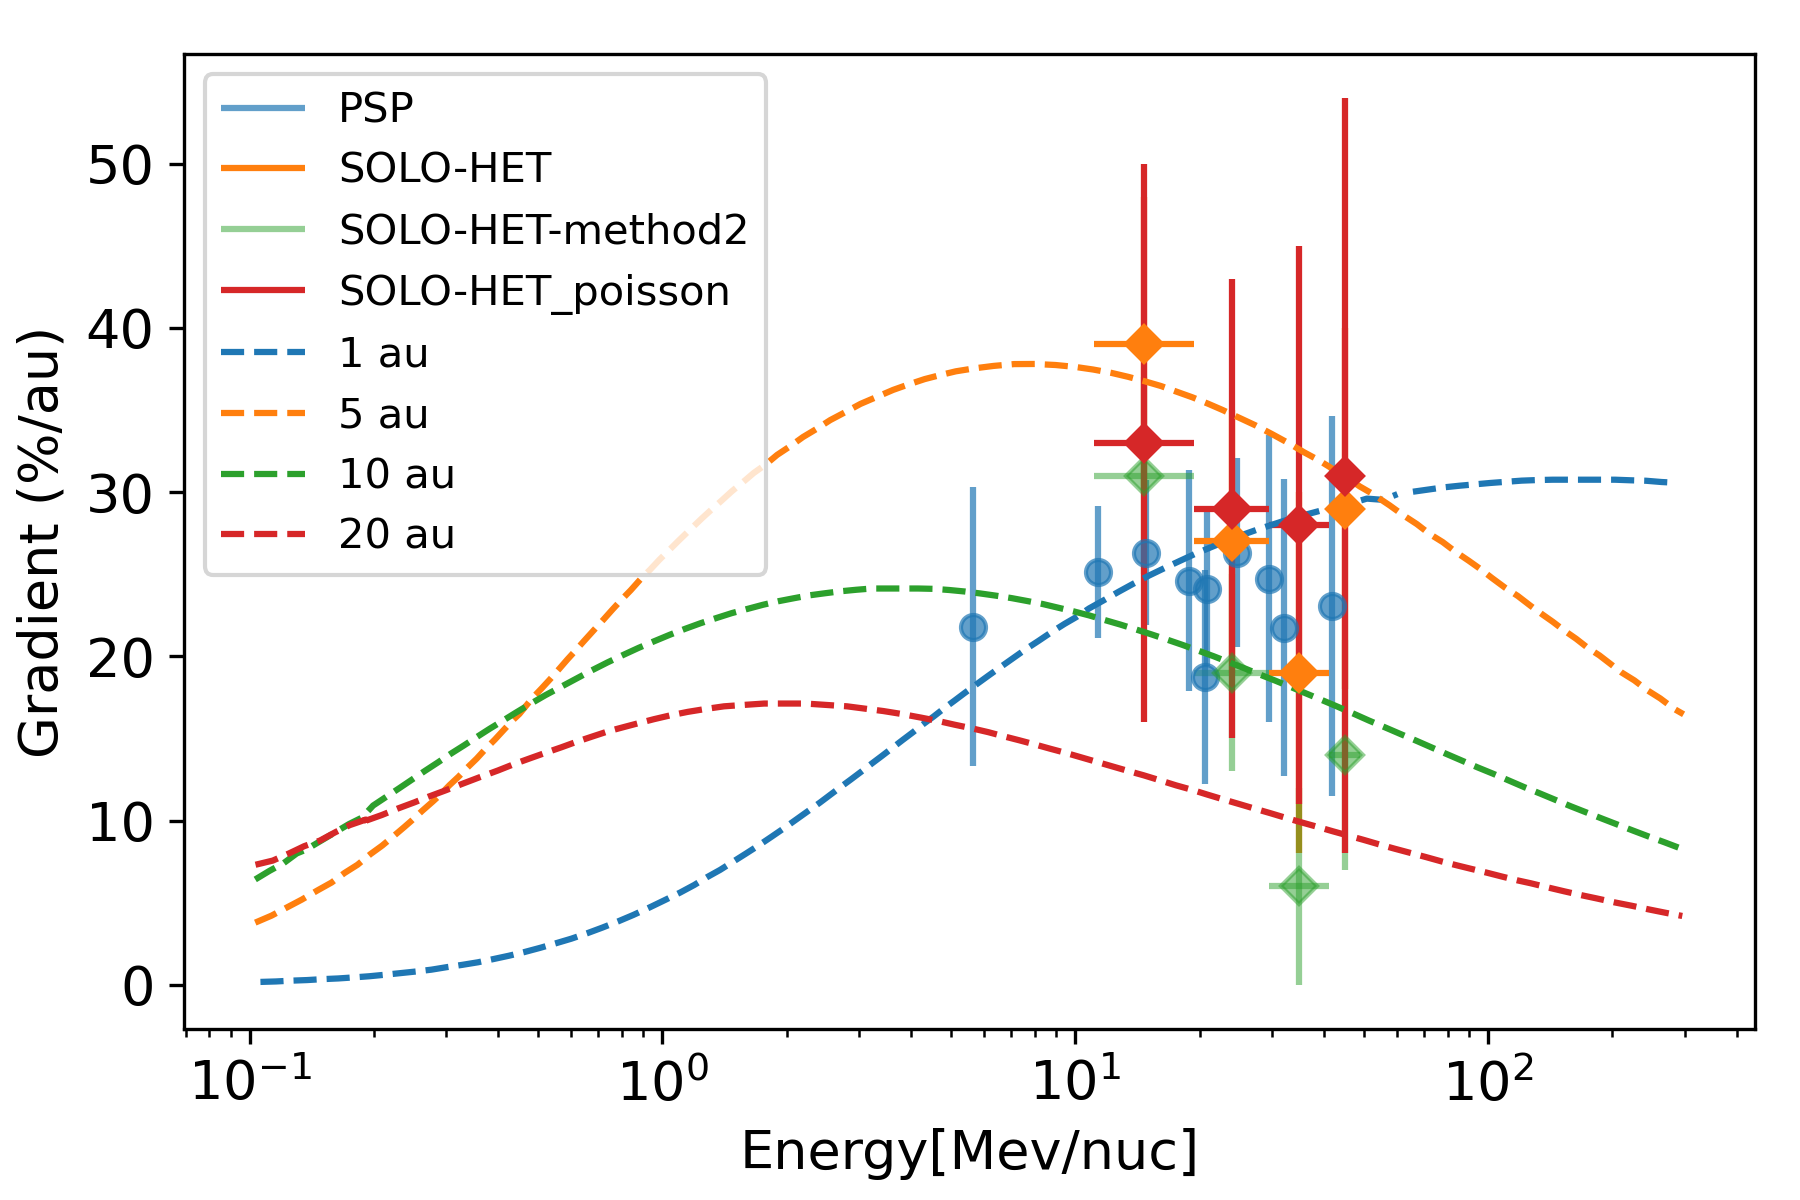
\includegraphics{images/ACR/Gradient_Energy_distribution_v2}
    \caption{The radial gradient of Helium measured on the ecliptic plane at different energies. The values (1 au) based on the SOLO/HET measurements are given as diamonds with corresponding error bars in orange (SEP-mask-Carrington-average), green (SEP-mask-daily-averaged), red (SEP-mask-larger-than-0.9-Poisson-distribution-80000s-daily). The dashed lines are generated based on the model \citep{Strauss&Potgieter_2010} \TODO{New simulation and ask help from some one in Kiel, not now}. We extracted the result from \citep{Rankin2021ApJ}.  \TODO{This image need to be reproduct, using just the one case}}
    \label{fig:comparison_SOLO_PSP}
\end{figure}


\subsection{The time variation of the radial gradient}


\section{Results and summary}

We reported the ACR helium (10 - 50MeV/nuc) measured by SolO/HET from 2020 - 2022.9. The first half period is still the solar minimum with almost no solar activities and the second half has increasing number of solar eruptions.
The comparison between the helium spectra of SOLO/HET, SOHO/EPHIN and ACE/SIS indicates a good agreement. SolO and ACE are also consistent with each other for Carbon, Oxygen and Nitrogen.
We removed the long-term solar modulation, SEPs, and short-term variation due to CIR from the temporal profile and derived the radial gradient of helium over energy ~10 - 50 MeV/nuc.
The radial gradients of 10 - 20 MeV/nuc are consistent in two methods which are also compariable to the PSP results.
Solar activities affect the radial gradient. It is difficult to derive the weak radial gradient when the intensity changed dramatically.
Currently, the results have larger uncertainties and more discussions are needed to improve the results.






%\input{chapters/pub04_xu2022}
